% Chapter 4

\chapter{Goanna: Finding All Type Errors Using Minimal Correction Sets} 

\label{chap:goanna} 
\graphicspath{{Figures/Goanna}}


In this chapter, we introduce Goanna, another Haskell type error debugging tool.  Goanna aims to provide a set of debugging utilities to support resolving multi-witness type errors and multi-party type errors. Goanna sets itself apart from both traditional tools and \chameleon{} through its unique features, such as identifying all potential causes of type errors, suggesting fixes, and supporting cross-module debugging. This chapter begins by highlighting the limitations of conventional compiler error messages and then details Goanna's capabilities in identifying and ranking potential causes by their likelihood. We then discuss the implementation strategies and heuristic methods employed in Goanna. Finally, we present an empirical evaluation of the system's accuracy, conciseness, and performance using real-world Haskell code examples.


 This chapter uses the content from our paper \textit{Goanna: Resolving Haskell Type Errors With Minimal Correction Subsets} \cite{Fu2024-rw}, with slight modifications to ensure coherence within this thesis. This work was under review for the International Conference on Function Programming (ICFP) 2024 at the time of submitting this thesis.



\section{Introduction} \label{sec:introduction}
    
Statically typed languages have gained popularity in the mainstream programming world \cite{StackOverflow2022-aw}. Many new languages have been designed with strict type systems, while others have introduced static typing through external tools. Numerous studies indicate that programming with statically typed languages can prevent certain errors \cite{Bogner2022-vf}, enhance code quality \cite{Mayer2012-lg}, and reduce maintenance costs \cite{Kleinschmager2012-bg} compared to similarly positioned dynamic languages \cite{Bogner2022-vf}. Despite their increasing popularity and benefits, challenges persist in the real-world adoption of these languages \cite{Zeng2019-ou}. The steep learning curve of complex type systems remains an obstacle to their adoption. 

Haskell is renowned for its expressive and robust type system. It enables programmers to model complex problems as constructs and relations within type systems and develop programs in a type-driven style. Historically, many type system innovations initially introduced by Haskell \cite{Hudak2007-kn}, including algebraic data types, type inference, and type classes, have now found their way into mainstream programming languages \cite{TypeScriptTeam_undated-qk,Klabnik_undated-mp,Griesemer_undated-ff}.
    
However, Haskell is also known for its steep learning curve and unforgiving type errors. Numerous research efforts have attempted to address these challenges \cite{Tirronen2015-nr,Chen2014-dz, Heeren2003-kd,Zhang2015-xy, Lerner2007-mu,Zhang2017-tj}. The type errors generated by the most commonly used Haskell compiler, GHC (Glasgow Haskell Compiler), often lead to confusion among novice users, and sometimes experts. For instance, in the program shown in Fig.~\ref{fig:motivation}, a type mismatch between a {\tt Char} type and an integer number type results in a perplexing type error for novice users. We have identified three challenges for making use of these error messages:


    \begin{enumerate}
        \item Fixated on one possible cause while other potential causes exist.
        \item Changing the suggested location does not completely rectify the error.
        \item Not enough contextual information for programmers to understand how the judgment was made.

    \end{enumerate}


    \begin{figure}[ht!]
        \centering
        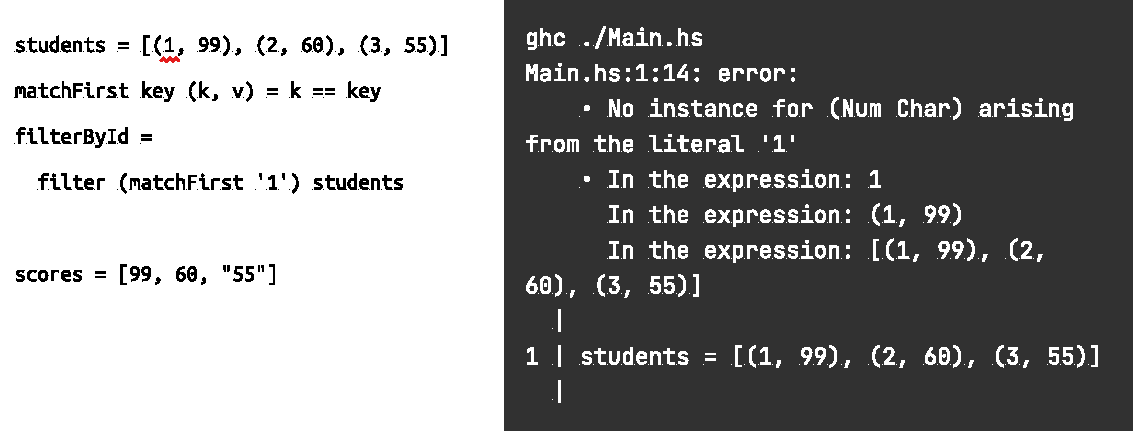
\includegraphics[width=\linewidth]{images/motivation}
        \caption{Inspecting a type error using the Haskell compiler GHC (Glasgow Haskell Compiler)}
        \label{fig:motivation}
    \end{figure}




    To address these challenges of diagnosing and fixing type errors in Haskell, we present a new tool: \textit{Goanna}. Goanna is a Haskell type checker based on Minimal Correct Subset (MCS) enumeration. Compared to traditional type-checking tools, Goanna provides improved type error reporting by giving a comprehensive list of possible causes and suggesting valid fixes for each cause.  Goanna differs from past type debugging systems (as reviewed in Section~\ref{sec:related-work}) through its use of Minimal Correction Subsets (MCS), where a single MCS represents a complete set of locations that constitutes a possible cause.

	To further enhance Goanna's support for type-error resolution, we provide optimization strategies (Section~\ref{sub:optimization}) to identify and reduce the unhelpful suggestions, as well as ranking heuristics (Section~\ref{sub:ranking}) to suggest more likely fixes first. Additionally, we provide Goanna-IDE, an interactive debugging front-end designed to efficiently navigate and interpret Goanna's type error diagnosis.

    We conducted empirical studies that evaluated Goanna's accuracy (Section~\ref{sub:eval-accuracy}), conciseness (Section~\ref{sub:eval-conciseness}), and performance (Section~\ref{sub:eval-performacne}). Our evaluation shows that compared to other type-checking tools, Goanna consistently provides accurate error diagnostics and correct fixes in its top suggestions. We also demonstrate that Goanna generally offers a concise list of possible causes, thanks to its cause optimization process. While Goanna may not consistently provide instantaneous results for real-time feedback, it can deliver on-demand diagnoses when programmers require additional assistance.
    

    The key contributions of this research include:
    \begin{itemize}
        \item Goanna, a Haskell type checker with improved error reporting based on MCS enumeration and program slicing;
        \item Goanna-IDE, an interactive type error debugging interface for Haskell; 
        \item A collection of heuristics and optimization techniques to enhance MCS-based type error reporting; and
        \item An evaluation of Goanna's accuracy, conciseness, and performance.
    \end{itemize}

  The techniques we used in Goanna, such as MCS enumeration and heuristics for ranking possible causes, are not exclusive to Haskell. Rather, they are applicable to statically typed programming languages in general. We intentionally designed Goanna to use a modular architecture that can be easily extended to support other programming languages with similar typing disciplines.


    \section{Goanna-IDE Walkthrough} \label{walkthrough}
    We first illustrate Goanna's capability by demonstrating the usage of Goanna-IDE. Goanna-IDE is a type error debugging interface for Haskell. It is designed to efficiently navigate and make use of Goanna's type error diagnosis through visualization and interactivity. Goanna-IDE provides comprehensive diagnostic error messages for type errors in Haskell and allows programmers to interactively explore their options. An online demo of Goanna-IDE is available for evaluation at \cite{Fu2023-bo}. Goanna-IDE includes a file explorer, a text editor, and a debugging panel. Goanna-IDE provides the following features when type errors are encountered:

    \begin{itemize}
        \item Thoroughly detect all type errors within the codebase and allow users to inspect each type error individually via the debugging panel.
        \item Indicate the most likely causes by star indicators.
        \item Show necessary type hints in the editor panel to help reason about each possible cause.
        \item Allow users to trace type errors across multiple files.
    \end{itemize}

    \subsection{Examples of Diagnosing Type Errors with Goanna-IDE}

    For the type error in the motivating example, Goanna shows 6 possible causes of the error (see top right corner of Fig.~\ref{fig:goanna-example-1}). When focussing on the cause suggested by GHC, instead of highlighting only the literal \texttt{1}, Goanna reports all 3 literals that needed to be changed all at once if the programmer chooses to address this cause. In addition, Goanna also indicates that these integer literals need to be changed to \texttt{Char} type using the inlay type hints on line 1, largely narrowing down the potential ideal fixes. 
    

    \begin{figure}[ht!]
        \centering
        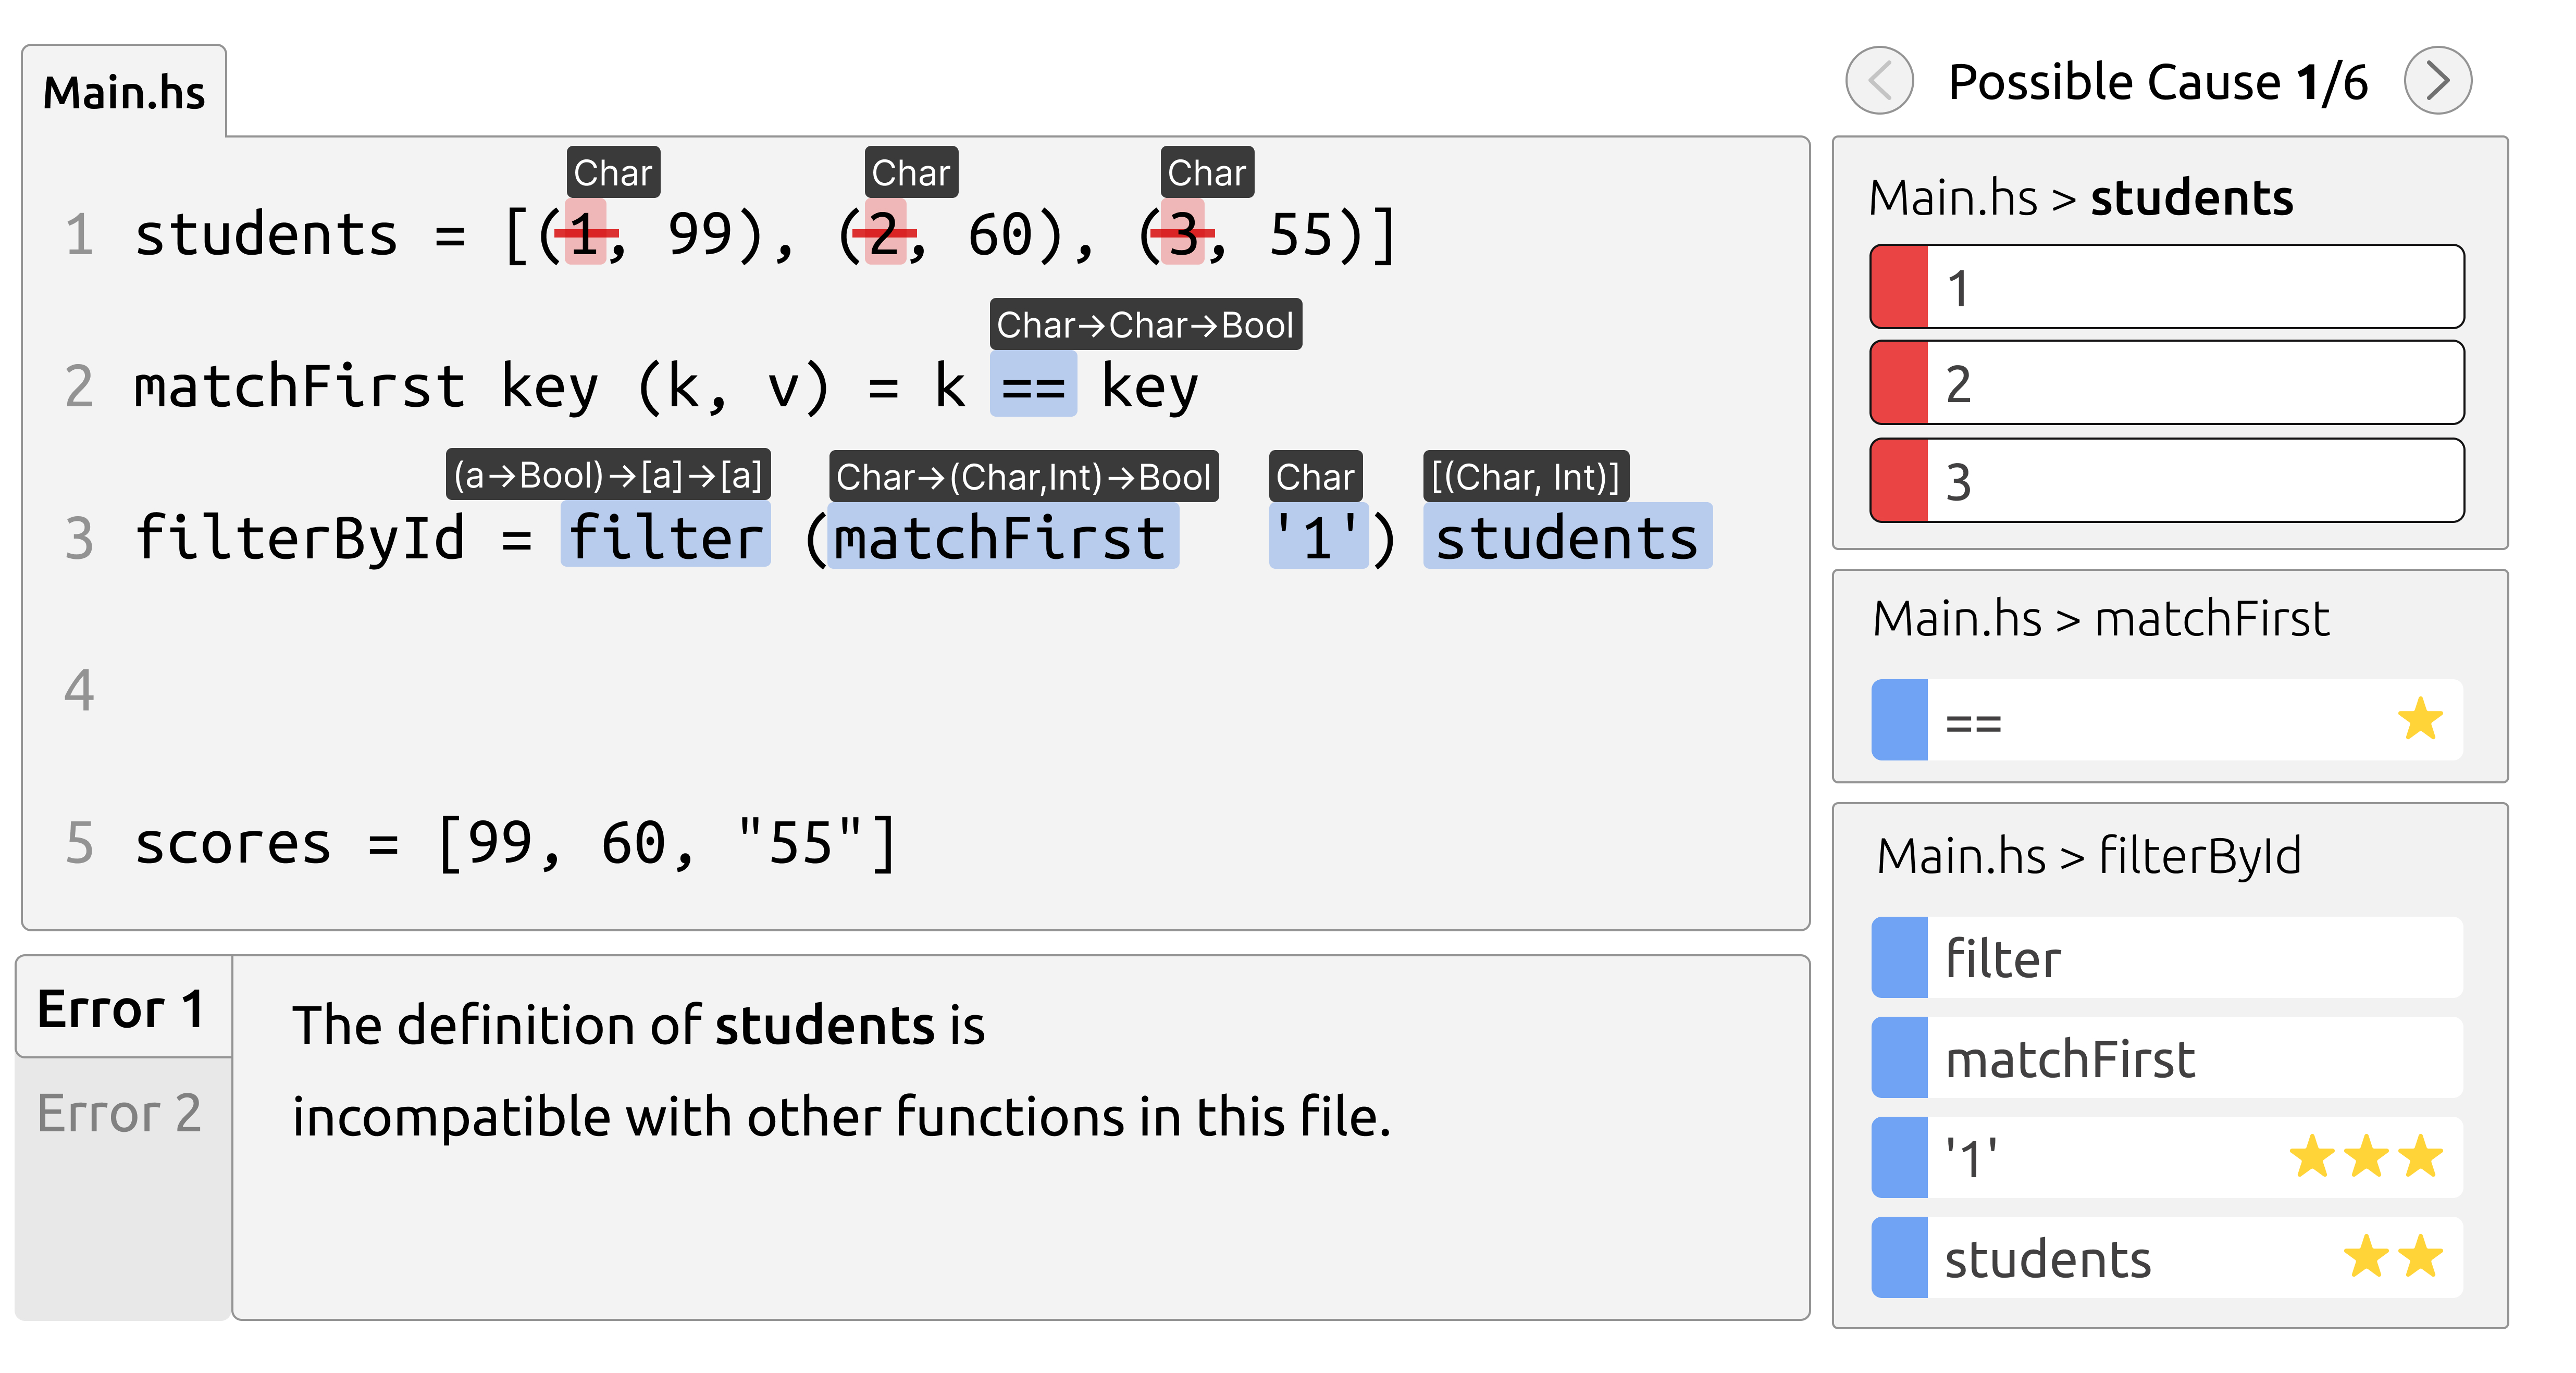
\includegraphics[width=\linewidth]{images/Goanna-Example-1}
        \caption[Goanna's showing possible causes of a type error (1)]{\textbf{Goanna's error diagnosis} Goanna shows that to fix the type error, the literals \texttt{1}, \texttt{2}, and \texttt{3} on line 1 need to be changed to Char type.}
        \label{fig:goanna-example-1}
    \end{figure}


    Note that the cause suggested by GHC is only one of the possibilities identified by Goanna. In fact, Goanna suggests that there are more likely fixes, indicated by the star symbols. The most likely fix, based on Goanna's cause heuristics (Section~\ref{sub:ranking}), is the \texttt{Char} literal \texttt{'1'} on line 5, indicated by the 3 stars (Fig.~\ref{fig:goanna-example-1}).
    
    
    By clicking on the most likely cause, Goanna shows different highlights in the editor (e.g., see Fig.~\ref{fig:goanna-example-2}). Goanna reports the error is caused by the literal \texttt{'1'} and suggests changing to an integer. All the type hints are adjusted based on our new assumption. Goanna ranks all possible causes using a series of heuristics. In this case, the preference is largely influenced by how many locations are required to change to fix the error. 
    
    \begin{figure}[ht!]
        \centering
        \includegraphics[width=\linewidth]{images/goanna-example-2}
        \caption[Goanna's showing possible causes of a type error (2)]{\textbf{Goanna's error diagnosis.} Goanna shows that the type error can be fixed by changing the literal $'1'$ on line 3, which needs an \texttt{Int} type. This, according to Goanna, is the most likely cause of the type error.}
        \label{fig:goanna-example-2}
    \end{figure}


    \subsection{Identifying all type errors} \label{sub:all-errors}
    
    A key feature of Goanna is its ability to detect all type errors in the code thanks to its MCS enumeration (Subsection \ref{sub:enumeration}). This is not always the case with other tools, such as GHC, which may only report a subset of the errors present in the code or stop at the first error they encounter. Goanna, however, always thoroughly identifies all type errors in the codebase. In the example of Fig.~\ref{fig:goanna-example-1} and Fig.~\ref{fig:goanna-example-2}, Goanna discovered the two errors included in the file. Clicking on the error selector on the bottom-left will change the content of the debugging panel and text editor highlights to reflect the cause of a different error (Fig.~\ref{fig:multi-error}). 

    \begin{figure}[ht!]
        \centering
        \includegraphics[width=\linewidth]{images/goanna-multi-error}
        \caption[Selecting a different error in Goanna]{\textbf{Selecting a different error in Goanna.} Selecting a different error using Goanna's error selector. The debugging panel will show potential cause locations for the selected error. The highlights and type hints in the editor panel will focus on the selected error.}
        \label{fig:multi-error}
    \end{figure}



    \subsection{Type error grouping}  \label{sub:group}
    In addition to reporting multiple errors, Goanna also groups together type errors that might be treated as separate by other tools. Goanna uses a novel approach (Section~\ref{sub:grouping}) to ensure that type errors that are intuitively connected are grouped together. This means that Goanna does not overwhelm the programmer with an excessive number of redundant type errors. Instead, the programmer is presented with a concise list of errors that all can be assessed separately.

    \begin{figure}[ht]
        \centering
        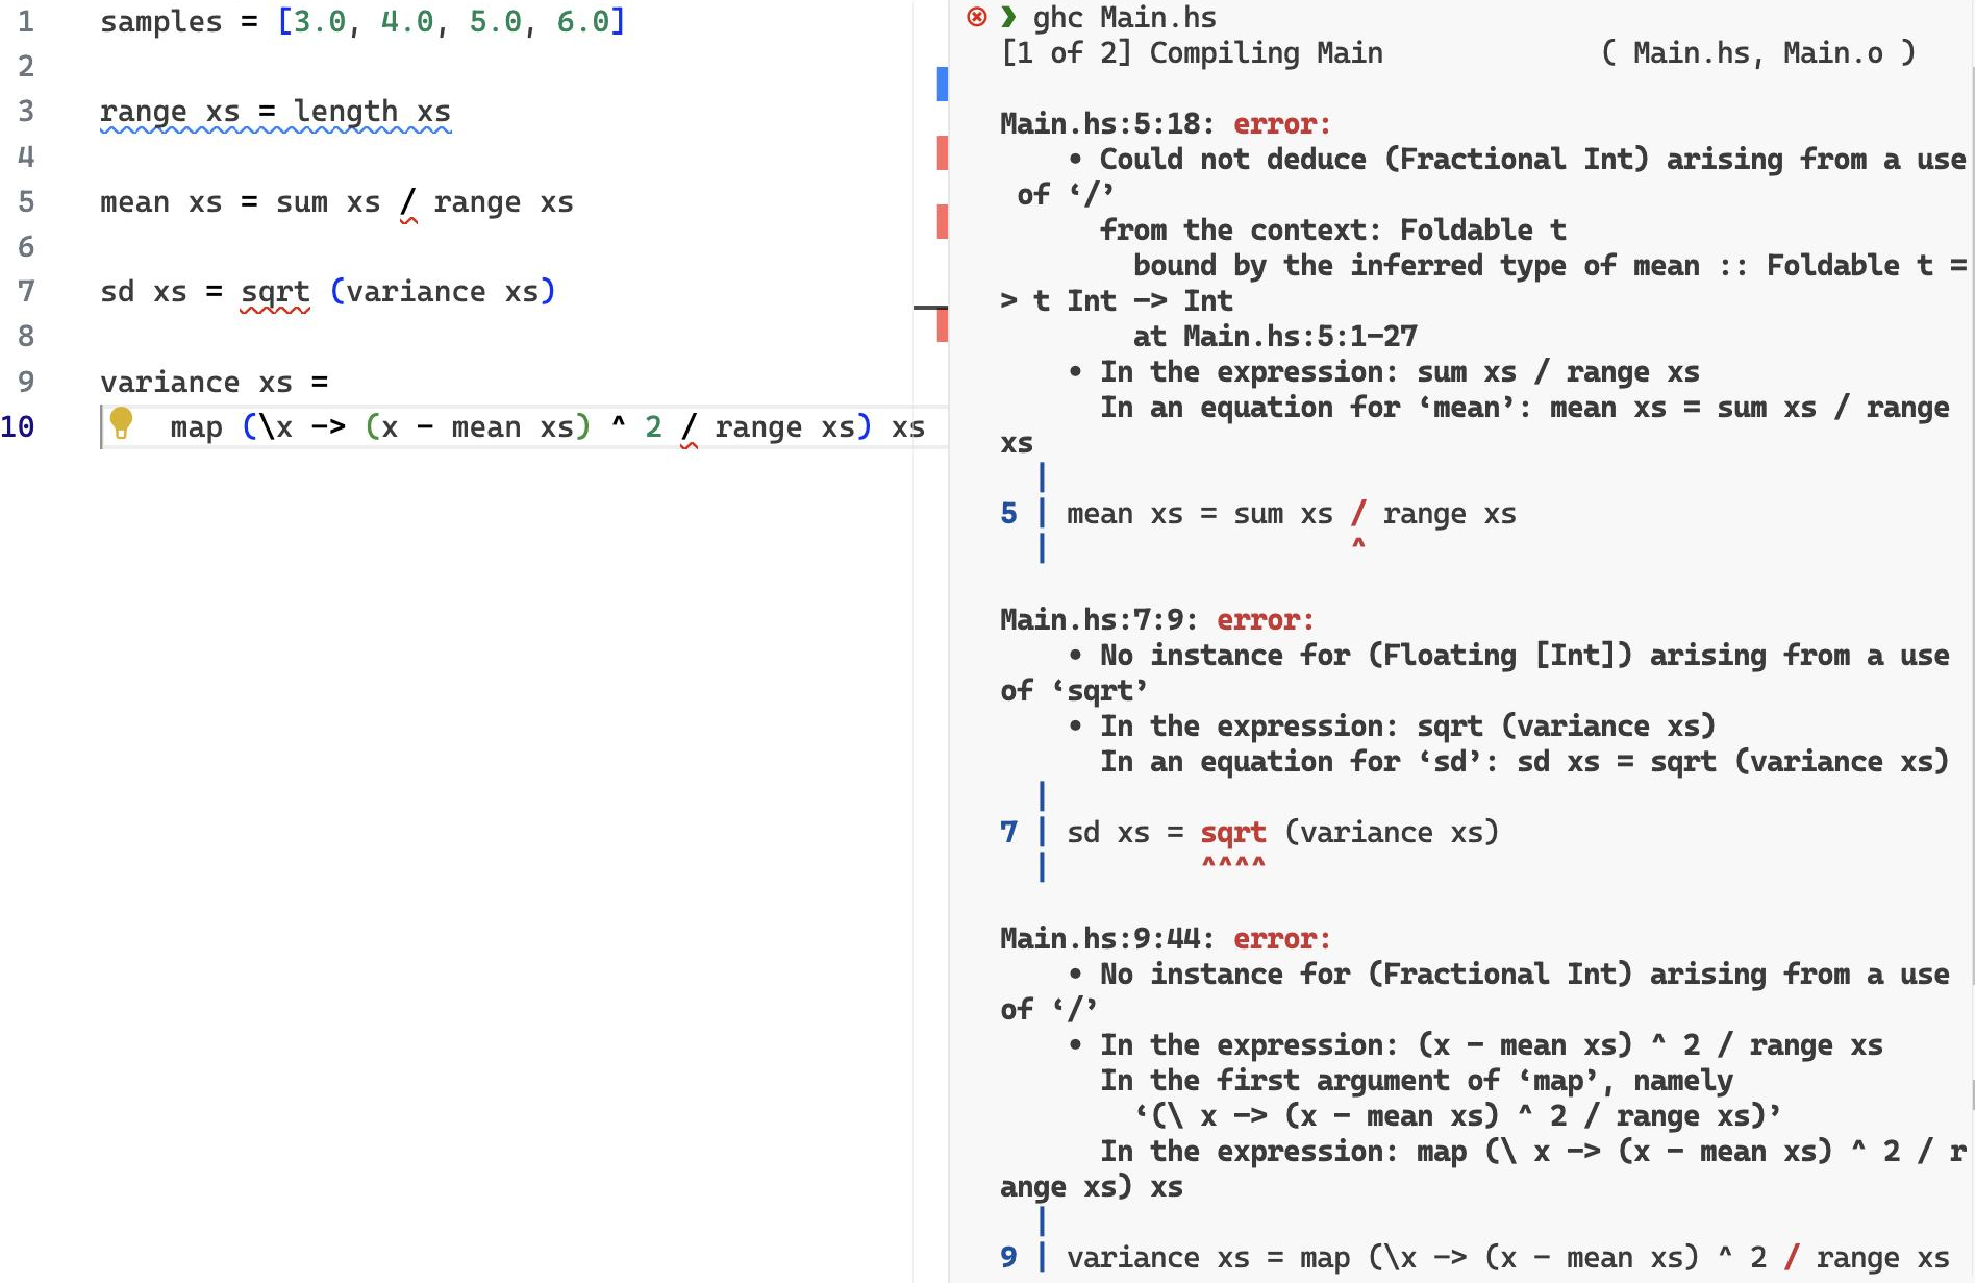
\includegraphics[width=\linewidth]{images/variance-ghc2}
        \caption[Inspecting a defective Haskell Program in relation to the error messages output by the standard GHC compiler]{\textbf{Inspecting a defective Haskell Program (left) in relation to the error messages output by the standard GHC compiler (right)} -- 3 separate type errors are reported.  The editor (VS Code is used here) underlines the error locations reported in the messages, but all other contextual information must be understood from the error text.}
        \label{fig:grouping-ghc}
    \end{figure}
    
        \begin{figure}[ht!]
        \centering
        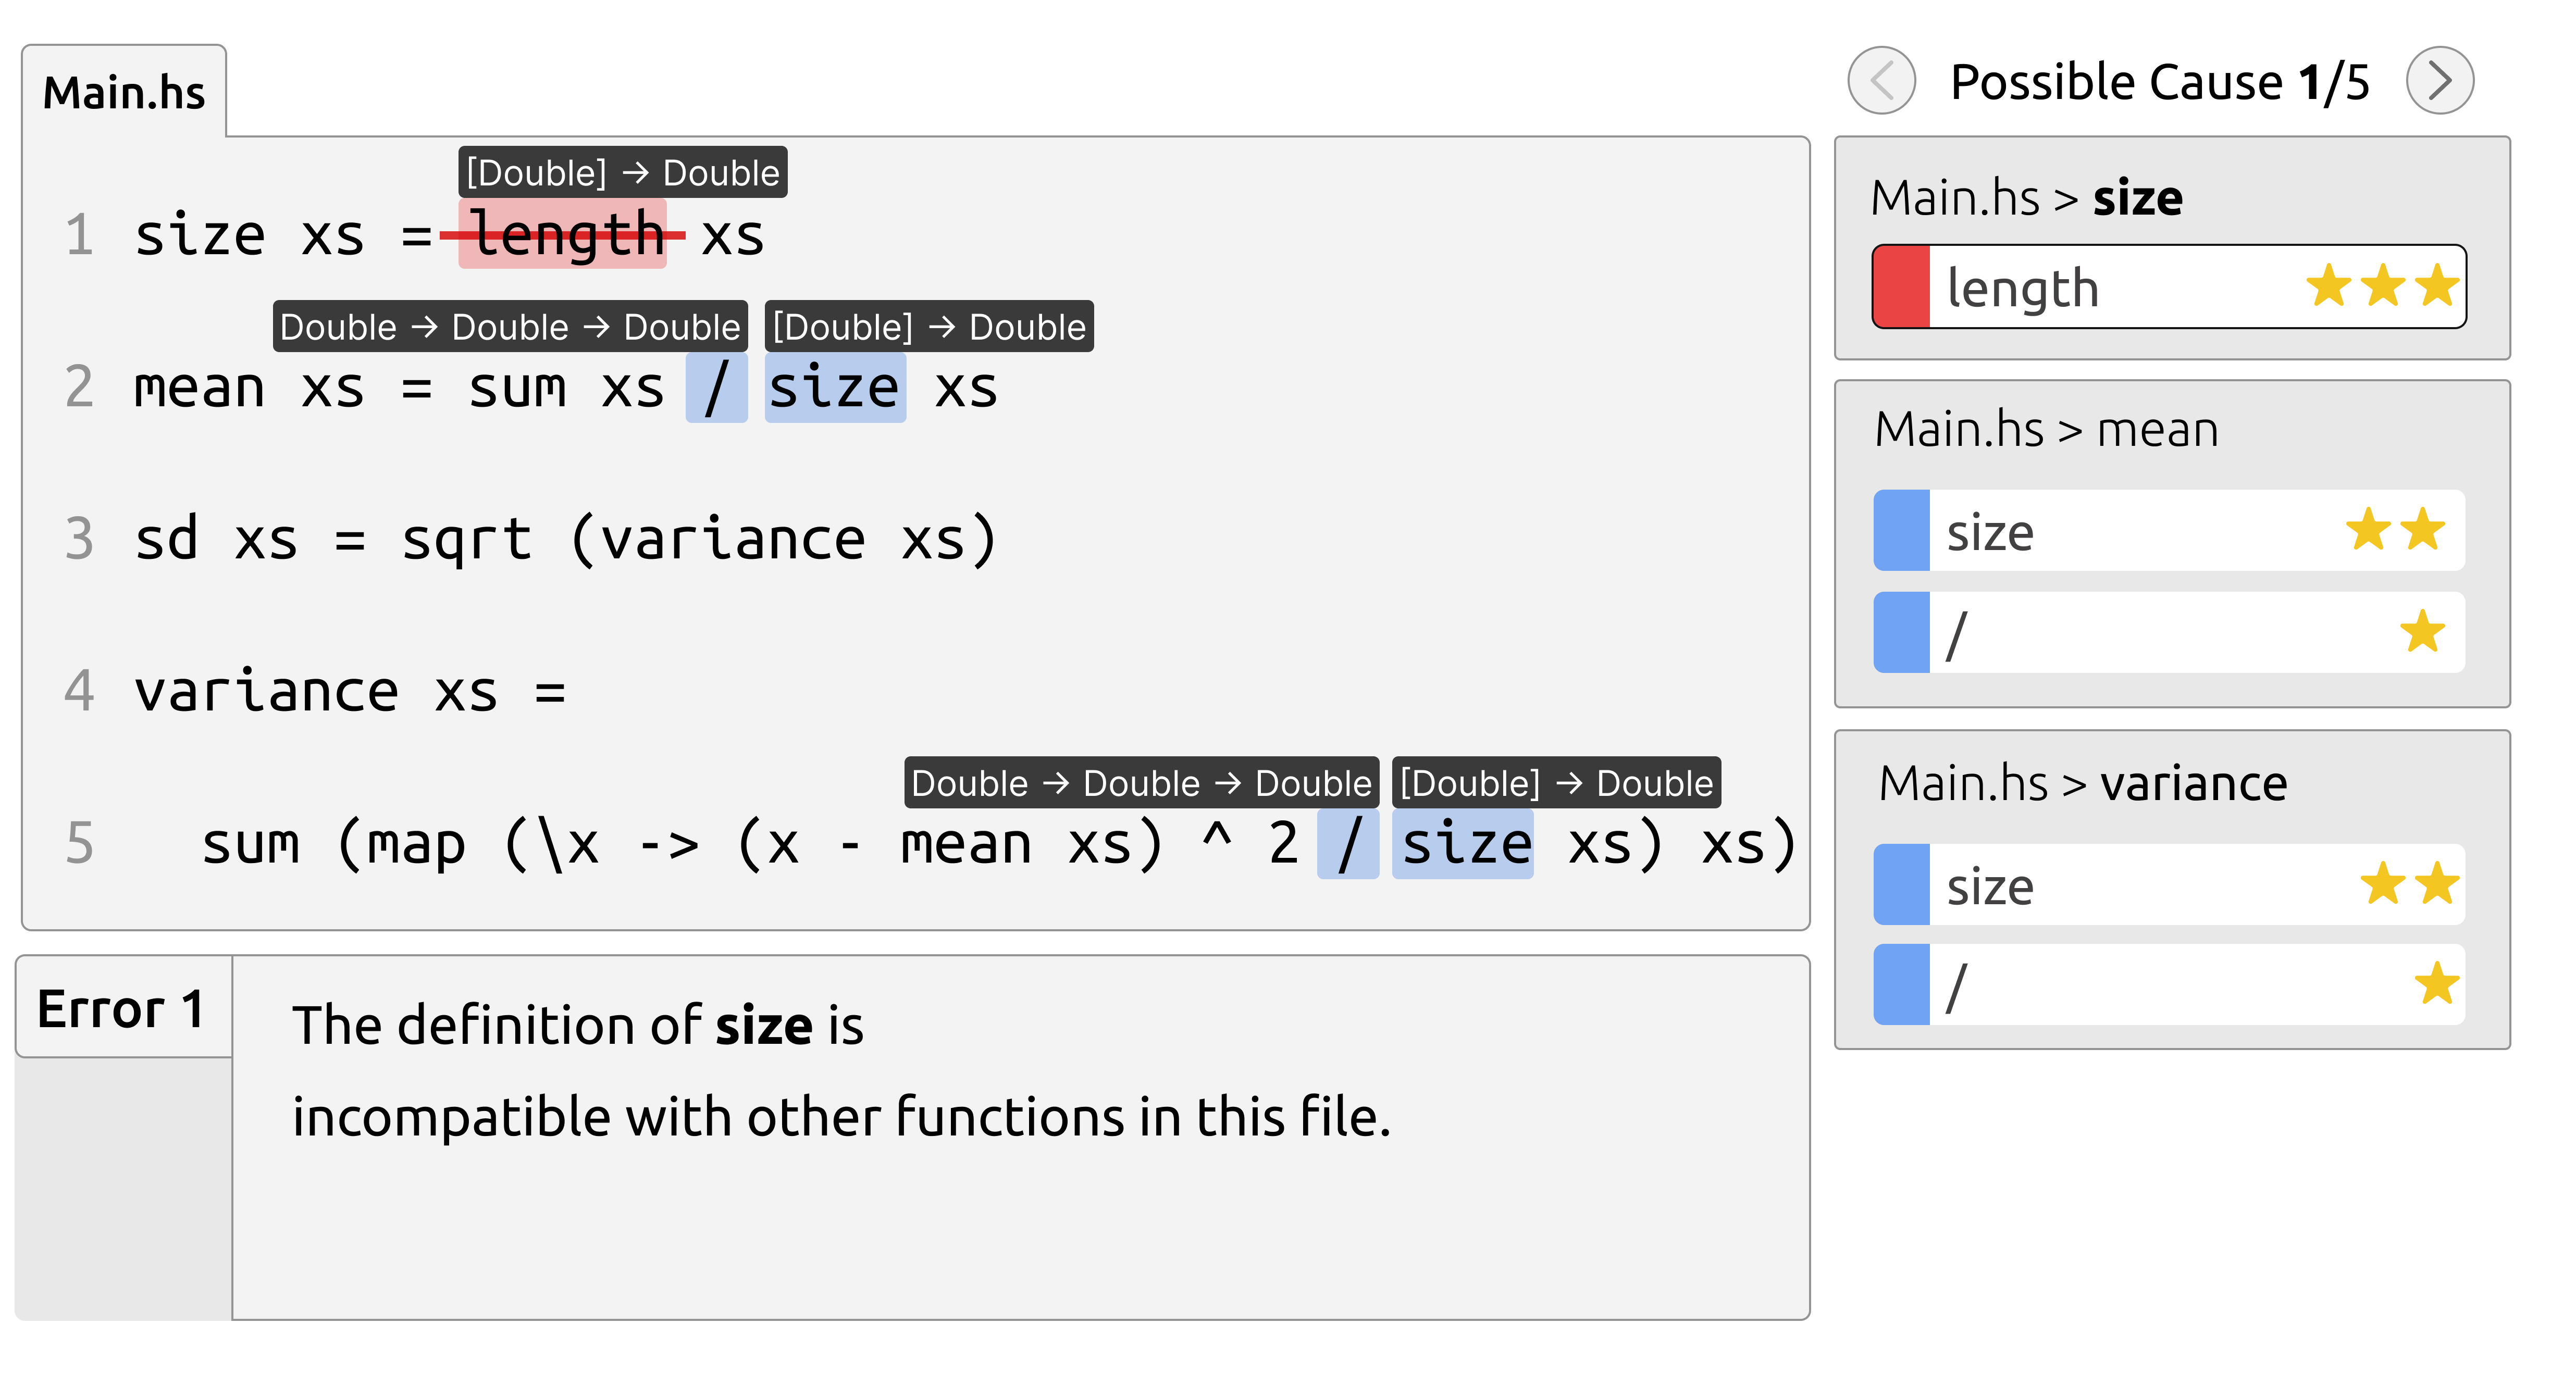
\includegraphics[width=\linewidth]{images/Goanna-Error-Grouping}
        \caption[Goanna's Error Grouping]{\textbf{Goanna's Error Grouping.} This error, although its potential offending parts appear in many declarations, is possible to fix in one place, i.e., by changing the definition of the \texttt{size} function on line 1. Therefore, Goanna reports it as a single error.}
        \label{fig:grouping-goanna}
    \end{figure}

    For instance, in Fig.~\ref{fig:grouping-ghc}, the functions \texttt{variance} and \texttt{mean} expect the final type of \texttt{size} to be a fractional value. However, the definition of \texttt{size} results in an integral value, which creates a conflict. While GHC shows three separate type errors, Goanna groups these interconnected errors into a single entity, as shown in Fig.~\ref{fig:grouping-goanna}. These errors can be addressed collectively, thereby improving the efficiency of the programmer.

    \subsection{Discovering Potential Causes} \label{sub:suggesting}
    When a type error arises, Goanna-IDE shows a list of possible causes in the debugging panel. Each possible cause consists of one or more locations in the code that require modification to rectify the type error. Clicking on a possible cause activates it. The locations are highlighted in the text editor, as well as inlay type hints suggesting the suitable type expected for that code slice. In the debugging panel, the activated cause is outlined with a red icon, while others are marked with a blue icon. 

    The causes identified by Goanna are comprehensive. Goanna will take into account potential causes in expressions, pattern matchings, type annotations, and type class constraints. Consequently, programmers will generally find the real cause by exploring Goanna's diagnosis. Unlike most Hindley-Milner~\cite{Damas1982-zw} based type inference, Goanna does not show a bias towards the unification order, thereby avoiding the left-to-right bias \cite{Chen2014-ev}. 
    
    Note that Goanna's fixes are sufficient to resolve the type error. Traditional tools often reveal a set of partial locations of a type error, leaving programmers to realize later that additional adjustments are needed for a complete resolution. Goanna, however, offers fixes that encompass a complete set of changes necessary for a resolution.


    \subsection{Assessing Likelihood of Causes} \label{sub:conciseness}
    One challenge of Goanna's ``find all causes" approach is the number of ways an error can occur can sometimes become too large to be useful in practice. Goanna employs multiple techniques to intelligently sieve the list. For the remaining list, Goanna employs a few heuristics to rank their likelihood and inform programmers which causes they consider first. 
    Goanna-IDE uses a star-based rating system to signal the ``likelihood'' of each cause. 3 stars indicating the most likely cause, 2 stars and 1 star follows. 

    \subsection{Type Hints}\label{subset:type-hints}
    In addition to suggesting which part causes that type error, Goanna-IDE explains why this is inferred by using in-situ type hints on necessary terms. The type hints are displayed as inlay decorations on top of respective fragments of source code. These type hints provide enough information for programmers to understand the type inference, and Goanna will leave out the terms that are irrelevant to the type error. Goanna's type hints are also dynamic to the selected cause. Programmers can observe how the inferred type of each term changes by changing the selected cause. Many modern programming tools use inlay type hints to support understanding, such as   Haskell Language Server~\cite{HLS-Developers2023-ot},  most often, these tools will display all type hints or none. Unlike in Goanna, these tools do not provide alternative sets of type hints for programmers to compare.
    
    \subsection{Cross-module type error debugging}\label{subsec:cross-module-type-error-debugging}
    When encountering a type error spanning across multiple modules, Goanna-IDE will group the potential causes indicated by their module and declaration block. Clicking on any possible cause location will focus the editor on the corresponding module (Fig.~\ref{fig:goanna-cross-module}). Goanna is the first tool to introduce cross-module type debugging. The way Goanna presents cross-module type errors is analogous to how run-time errors are presented in most programming languages. When encountering a run-time error, most programming environments show a call stack containing multiple file paths, and programmers can choose which file to start investigating. Often, programmers choose to start from the file authored by themselves instead of library files. Goanna uses this mental model to group potential locations that cause a type error by module and definition blocks. 
    
    \begin{figure}[ht!]
        \centering
        \includegraphics[width=\linewidth]{images/goanna-cross-module}
        \caption[Debugging a cross-module error in Goanna]{\textbf{Debugging a cross-module error in Goanna.} In this error, potential defects may appear in either module \texttt{A} and \texttt{B}. Goanna suggests 3 potential causes and fixes: 1) Change the type annotation of \texttt{x} to \texttt{[Maybe Int]} (Top). 2) Change the y variable on line 4 of module \texttt{A} to an instance of \texttt{Int}. 3) Change both the elements in the list literal in module \texttt{B} (Bottom), hence affecting the type of \texttt{y}. Clicking on each potential cause in the debugging panel results in different highlights and type hints in the editor panel.}
        \label{fig:goanna-cross-module}
    \end{figure}



    \section{Goanna Implementation} \label{sec:implementation}
    Goanna comprises 3 phases: constraint generation, MCS enumeration, and post-analysis. In the constraint generation phase, Goanna walks the abstract syntax tree and collects constraints. In the MCS enumeration phase, Goanna enumerates through all MCSes. Lastly, in the post-analysis phase, Goanna applies multiple optimization techniques to reduce the number of MCSes, group MCSes by common properties, and sort them based on heuristics.

    \subsection{Haskell Coverage}
    Goanna supports a wide and growing range of the Haskell 2010 language syntax \cite{Simon_Marlow2010-lg}. At the time of writing, fully supported features include module import/export, qualified imports, import hiding, do notation, algebraic data types, newtypes, type synonyms, type classes, operator sectioning, and range expression. Goanna does not yet support type features enabled through language extensions. However, they are also on the roadmap. A detailed and updated feature coverage \cite{Fu2023-rp} is publicly available.

    \subsection{Constraint Generation} \label{sub:translation}
    Goanna uses the abstract syntax tree of the original Haskell program and translates it into a constraint program by modeling how types are defined and used. Goanna does not restrict which constraint language and solver should be used. The only requirement is that Goanna needs to be able to assert whether a subset of the constraints is still feasible by calling a provided \texttt{solve} function during the MCS enumeration phase. In our implementation, we generate portable Prolog predicates \cite{Wielemaker2011-sr}. The \texttt{solve} function executes a predefined predicate \texttt{type\_check/0} that tests all the generated predicates. We used standard Prolog notation \texttt{name/arity} here when referring to Prolog predicates, as a Prolog predicate is identified by the combination of both attributes. 

    
    For a simplified Haskell syntax shown in Fig.~\ref{fig:translation}.A, we generate a list of Prolog predicates in the language shown in Fig.~\ref{fig:translation}.B. We use 3 auxiliary functions during the constraint translation process (Fig.~\ref{fig:translation}.C) to generate Prolog variables for future unification. \texttt{fresh} makes a unique unbound Prolog variable. \texttt{var} takes a Haskell identifier name and returns a Prolog variable. Naively, this can be done by turning it to uppercase. \texttt{atom} takes a Haskell type constant/constructor name and returns a Prolog atom. Naively, this can be achieved by turning it into lowercase. A global variable $\mathcal{P}$ is defined to store the list of predicates being generated. To clarify, all \textcolor{blue}{parsed Haskell syntax} aaare in blue. All \textcolor{red}{generated Prolog syntax} are in red. 
    
    Let $\Gamma$ be an open-ended list of Prolog atoms, containing names of Haskell local variables. Two sets of generation rule are defined to convert different Haskell syntax nodes to Prolog text. Predicate generation rules (Fig.~\ref{fig:translation}.D) take $\Gamma$ and Haskell declarations as input and output Prolog predicates. For example, a Haskell function \texttt{f = 2}, Goanna may generate a predicate \texttt{\textcolor{red}{f(V, \_) <- V = int.}}
    
    Constraint generation rules (Fig.~\ref{fig:translation}.E) take $\Gamma$, a Haskell expression node or type node, and a Prolog variable \texttt{V} as input and output a list of Prolog terms. These terms attempt to unify the inferred type of provided node to the provided Prolog variable \texttt{V}.
    
    \begin{figure}[ht!]
        \centering
        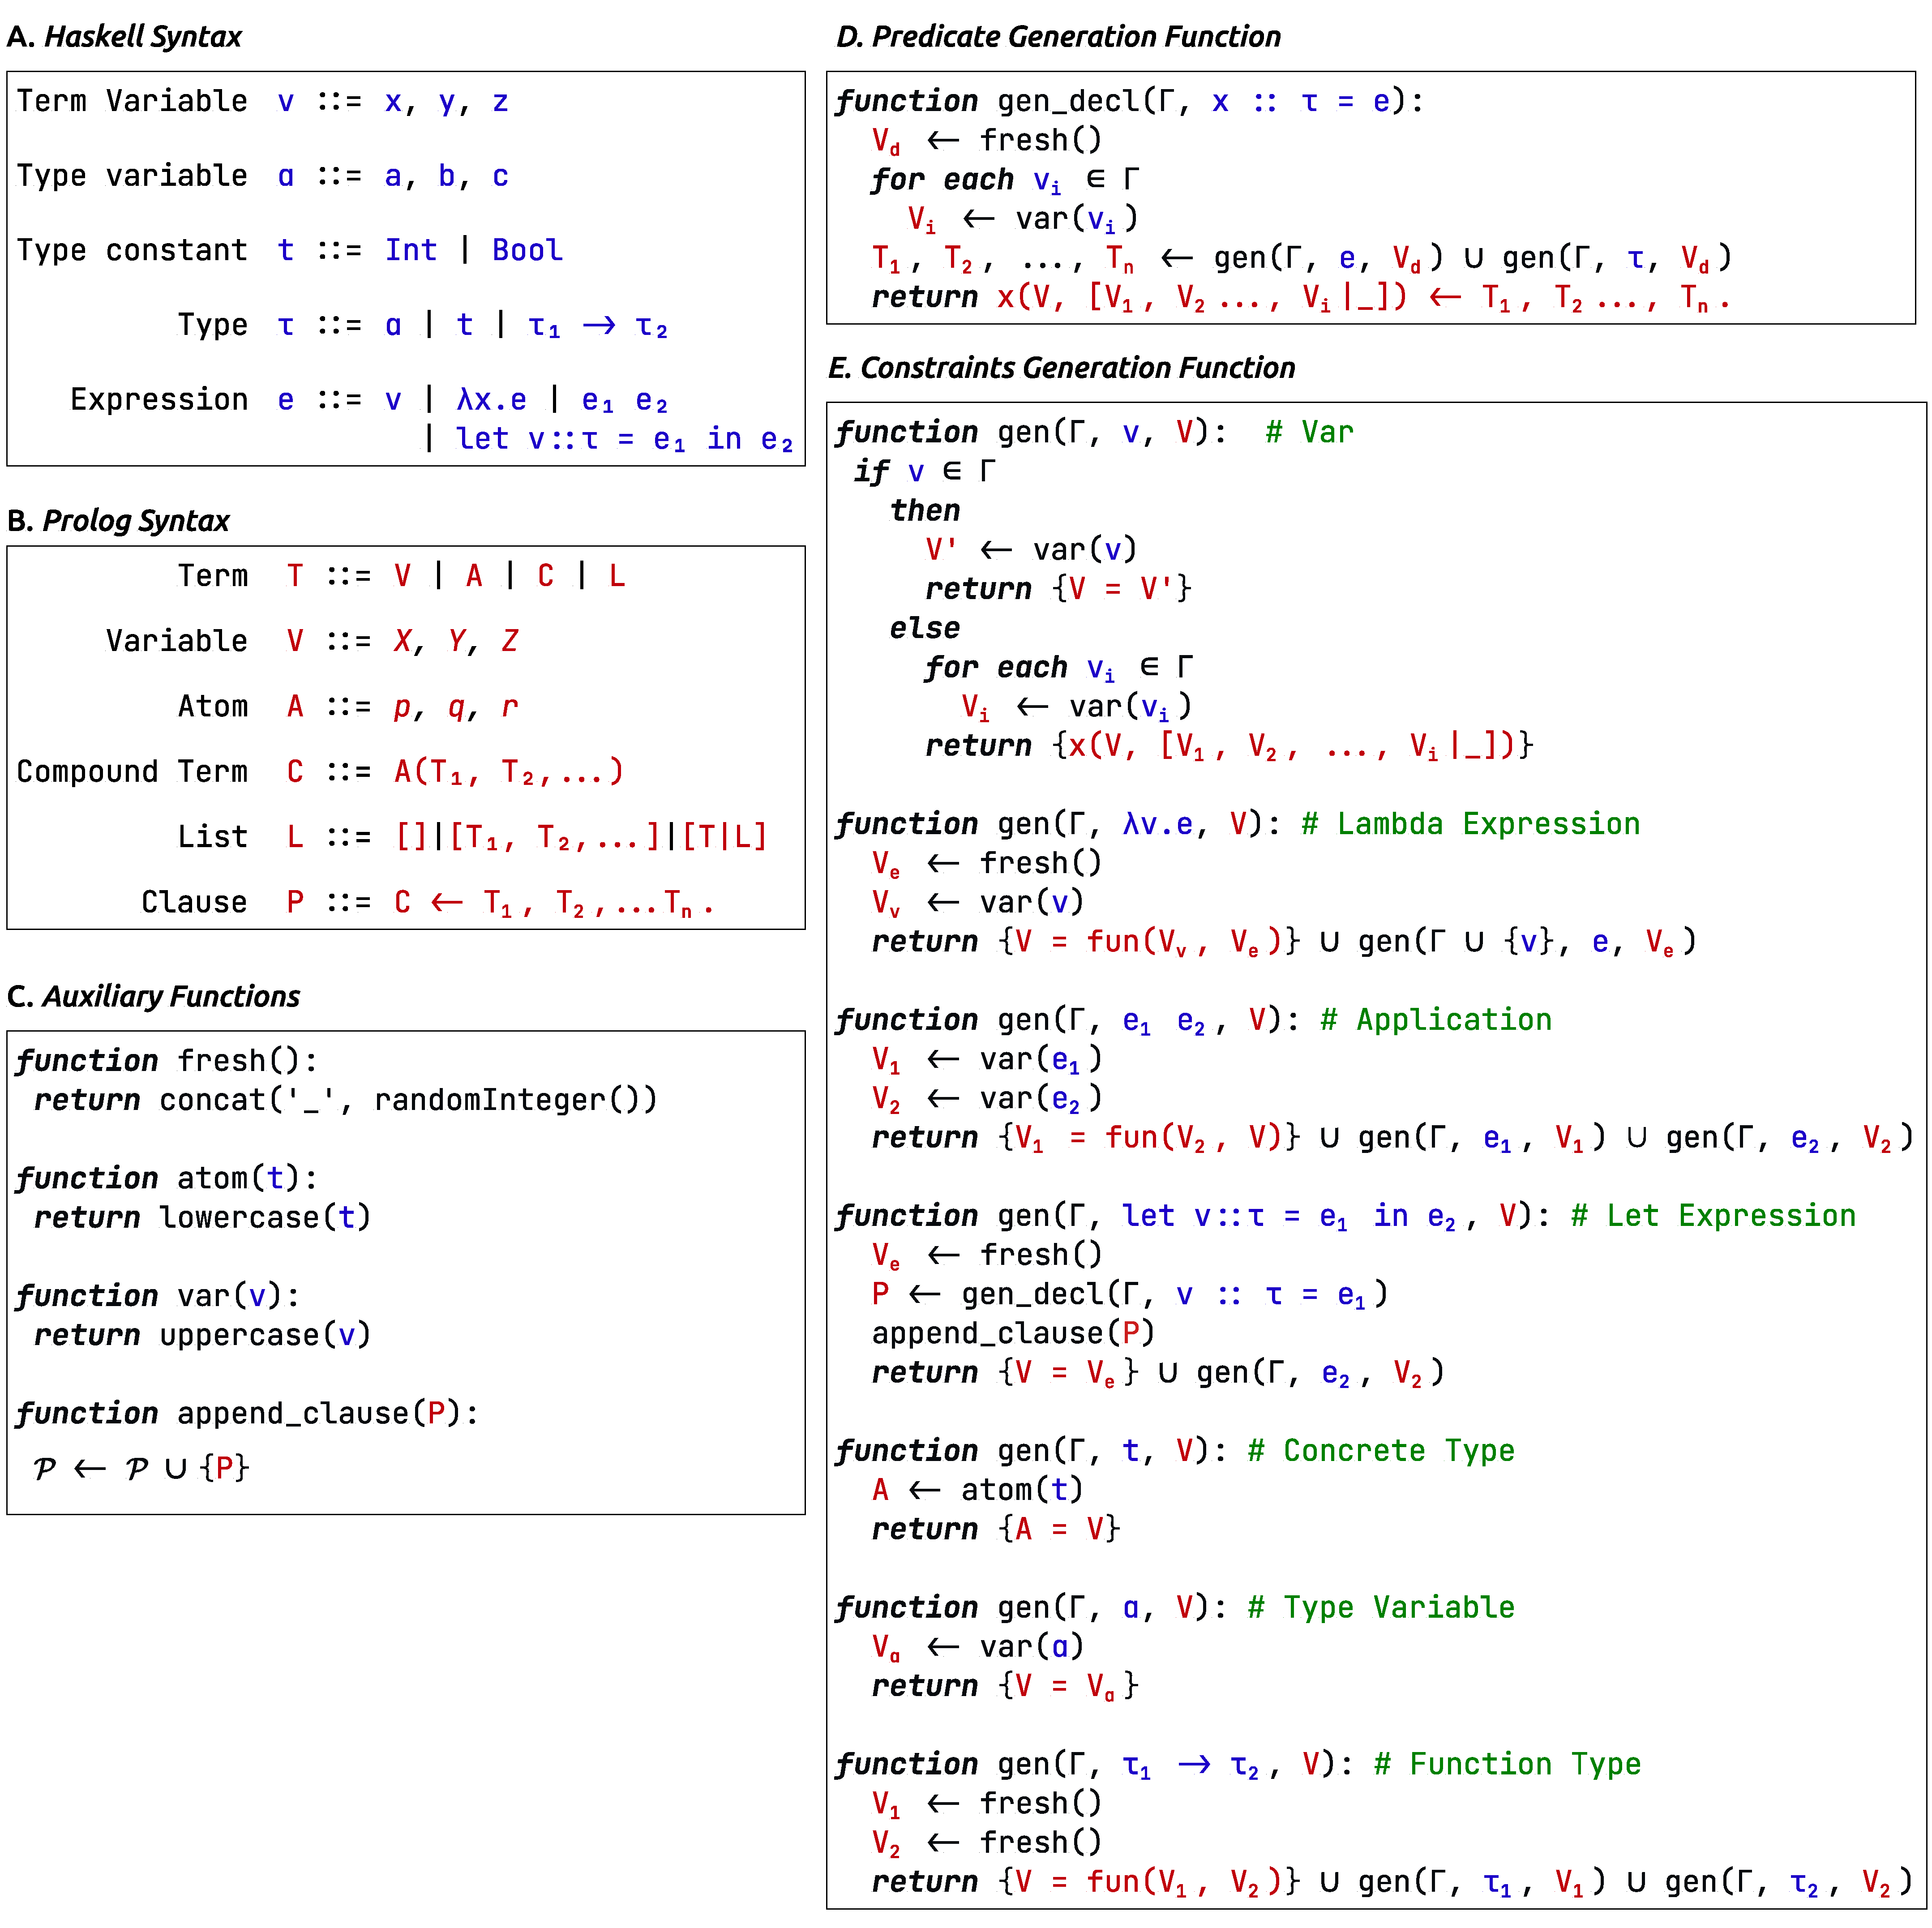
\includegraphics[width=\linewidth,trim={0 0.5cm 0 0},clip]{images/Generation2}
        \caption{Goanna's Constraint Translation Rules (Simplified)} 
        \label{fig:translation}
    \end{figure}
    
  
    An example of such translation can be found in Fig.~\ref{fig:translation-example}. In the Haskell program (Fig.~\ref{fig:translation-example}.A), 2 functions are declared: \texttt{f} and \texttt{g}. This will generate two corresponding Prolog predicates \texttt{f/2} and \texttt{g/2}. In the actual implementation of Goanna, the generated predicates would be \texttt{f/6} and \texttt{g/6}. The extra arguments are added to perform various tasks involving syncing state, such as breaking recursive calls and collecting type class constraints. In a predefined predicate \texttt{type\_check/0}, the subgoals \texttt{f(\_,\_)} and \texttt{g(\_,\_)} are added. Executing the top-level goal \texttt{type\_check} in a Prolog environment will get a result of \texttt{false}.
    
  \begin{figure}[htb]
        \centering
    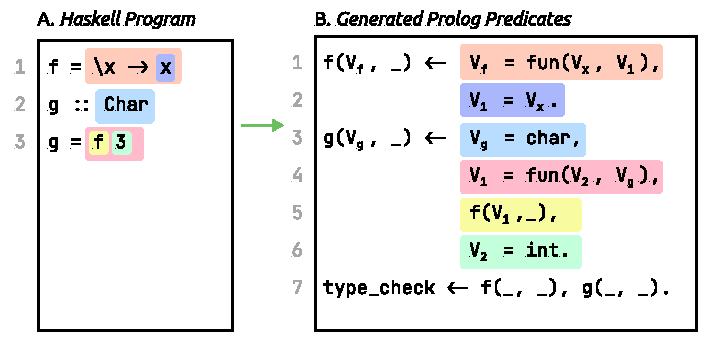
\includegraphics[width=0.7\linewidth]{images/Translation-Example}
        \caption[An example of Goanna constraint generation]{\textbf{An example of Goanna constraint generation.} For the Haskell functions \texttt{f} and \texttt{g}, Goanna generates the predicates \texttt{f/2} and \texttt{g/2}. Each subgoal of \texttt{f/2} and \texttt{g/2} is generated from a corresponding part of the Haskell program. In a predefined predicate \texttt{type\_check/0}, the subgoals \texttt{f(\_,\_)} and \texttt{g(\_,\_)} are added. Running the goal \texttt{type\_check} will return whether the program is well-typed. In this particular example, this will return \texttt{false}. We used standard Prolog notation \texttt{name/arity} here when referring to Prolog predicates, as a Prolog predicate is identified by the combination of both attribute. 
}
        \label{fig:translation-example}
    \end{figure}
    

    \subsection{MCS enumeration} \label{sub:enumeration}
    After the constraint generation phase, Goanna obtains a list of constraints derived from the source code and is able to query the feasibility of any subset of the constraint system by calling the \texttt{solve} function. Using a known algorithm \cite{Liffiton2016-xi}, Goanna then derives some useful subsets of the constraint system through MCS enumeration. We refer to the complete set of constraints as a constraint system $C$. When we use the word subset without specifying the corresponding superset, it can be inferred as the subset of the constraint system $C$. We list these subsets obtained from MCS enumeration and give their type-theoretic interpretation. 
    
        
    – A minimal unsatisfiable subset (MUS) $M$ of a constraint system $C$ is a subset $M \subseteq C$ such that $M$ is unsatisfiable and $ \forall{c} \in M : M \setminus \{c\}$ is satisfiable. An MUS can be seen as a minimal explanation of the constraint system’s infeasibility. MUSes have been used extensively, mostly in combination with programming slicing, as a means to explain type errors. A MUS of type system constraints reasoning chain connecting all evidence from one location of the conflict to another. Goanna uses the set of all MUSes to group related type errors.

    – A minimal correction set (MCS) $M$ of a constraint system $C$ is a subset $M \subseteq C$ such that $C \setminus M$ is satisfiable and $\forall{S} \subset M : C \setminus S$ is unsatisfiable. MCSes are so named due to the fact that their removal from $C$ can be seen to “correct” the infeasibility. In an ill-typed program, an MCS $C$ can be seen as the ``cause" of a type error; the removal of C will result in the system being well-typed. Goanna uses MCS to represent potential causes of a type error. Each MCS contains the set of locations that need to be changed to fully resolve the type error.
    
  – A maximal satisfiable subset (MSS) $M$ of a constraint system $C$ is a subset $M \subseteq C$ such that M is satisfiable and $\forall{c}\ in\ C \setminus M:M\cup\{c\}$ is unsatisfiable. The definition of an MSS is symmetric to that of a MUS, with “satisfiable” and “unsatisfiable” swapped along with maximal for minimal. MCS and MSS are the complement sets of one another. In an ill-typed program, an MSS $M$ can be seen as the resulting typing environment if a type error is fixed by excluding the MCS $C - M$. Goanna uses an MSS to provide type hints for the program even when it is ill-typed.
  
%  MCS enumeration has been previously studied for its application in error detection and fault identifications \cite{bekkouche_exploration_2015,lamraoui_formula-based_2016}. And the techniques of MCS enumeration have been improved through many studies \cite{liffiton_fast_2016,zhao_parallelizing_2016,bendik_must_2020}. Unlike previous tools \cite{stuckey_interactive_2003,haack_type_2004}, which use a single MUS, Goanna is the first to use MCS enumeration -- deriving all MUSes, MSSes, and MCSes -- in type error detection and localization. Goanna uses an implementation of the MARCO \cite{Liffiton2016-xi} algorithm to enumerate all MCSes.

 
     \begin{figure}[ht!]
        \centering
        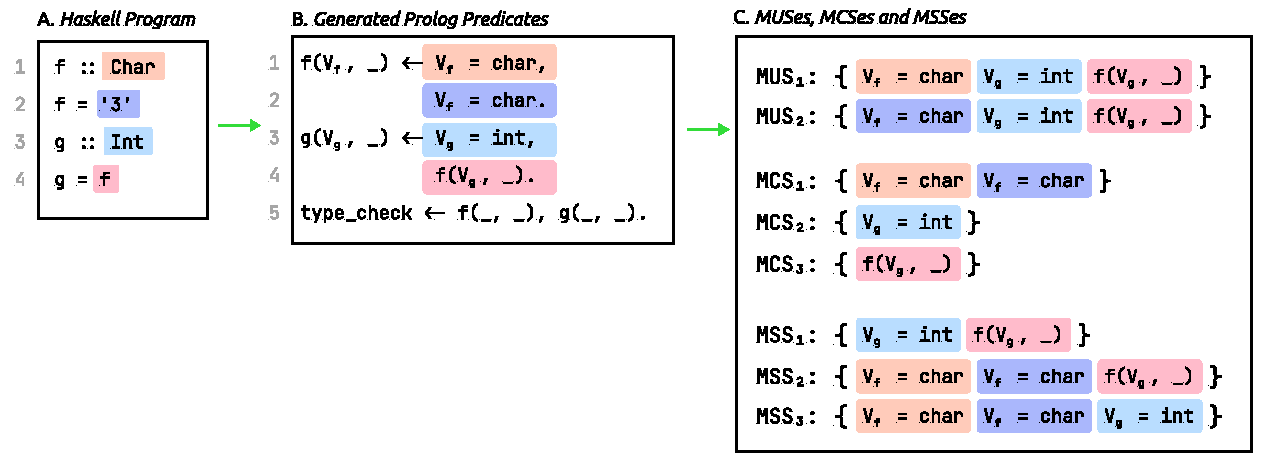
\includegraphics[width=\linewidth]{images/Enumeration-Example}
        \caption[An example of Goanna MCS Enumeration]{\textbf{An example of Goanna MCS Enumeration.} From the set of constraints (B) generated from the Haskell program(A), Goanna obtained 2 MUSes, 3 MCSes, and 3 MSSes. }
        \label{fig:enumeration-example}
    \end{figure}
    
   For the example in Fig.~\ref{fig:enumeration-example}, Goanna's MCS enumeration system identifies 2 MUSes, 3 MCSes, and 3 MSSes. Following the 3 MCSes, Goanna reports 3 potential causes of the type error: the type annotation and function definition in \texttt{f} (from $MCS_1$), the type annotation alone in \texttt{g} (from $MCS_2$), and the function definition alone in \texttt{g} (from $MCS_3$). 
   
   %    \[
%        \begin{array}{c}
%            MUSes = \{\{4, 8\}, \{6, 8\}, \{8, 10\} \} \\
%            MCSes = \{\{8\}, \{4, 6, 10\}\}            \\
%            MSSes = \{\{1,2,3,4,5,6,7,9,10,11,12\},\{1,2,3,5,7,8,9,11,12\}\}
%        \end{array}
%    \]
%
%
%    In the example shown in Fig.~\ref{fig:translation}, Goanna suggests two possible fixes: Fix 1 is represented by the MCS ${8}$, and the resulting types are inferred from the MSS ${1,2,3,4,5,6,7,9,10,11,12}$. Fix 2 is represented by the MCS ${4, 6, 10}$, and the resulting type is inferred from the MSS ${1,2,3,5,7,8,9,11,12}$.

%    \subsection{Improvement over MUS-based type error slicing} \label{sub:vs-slicing}
%    In conventional program slicing approaches, a Minimal Unsatisfiable Subset (MUS) is typically used to represent a single type error, thereby providing locations for the type error report. However, we have identified two significant limitations inherent in MUS-based localization and diagnosis:
%
%    \paragraph{Type error localization based on a single MUS only present partial evidence}
%    The minimality of MUS necessitates its exclusion of constraints leading to the same unification. Consequently, MUS-based tools often overlook certain evidence in the code that appears redundant. Programmers, however, are typically interested in obtaining an intuitive understanding of a program defect, not merely a concise proof. For instance, in the program illustrated in the listing \ref{listing:functionf}, MUS-based type error reporting would identify the conflict between the Char literal pattern and one of the three Integer patterns. However, it overlooks the crucial fact that three instances are suggesting \texttt{f:: Num a => String -> a}, while only one suggests \texttt{f::Num a => Char -> a}. With the knowledge of all MUSes, Goanna understands that the constraint that restricts the argument to be of \texttt{Char} type is present in all three MUSes. This allows Goanna to address the discrepancy of evidence in its fix suggestions.
%    \begin{lstlisting}[language=Haskell, caption={An erroneous function definition},captionpos=b, label={listing:functionf} ]
%f "A" = 1
%f "B" = 2
%f 'C' = 3
%f "D" = 4
%    \end{lstlisting}
%
%    \paragraph{Limited Reduction Capability of Single MUS-Based Type Error Localization}
%    MUS-based error slicing can effectively eliminate program locations that are not contributing to a type error. However, research indicates that program slicing can effectively reduce only around 30\% of the code size that is required to understand a type error \cite{binkley_empirical_2007}. Further reduction is challenging with the knowledge of MUS alone due to the MUS's minimality. For instance, in the code shown in listing \ref{listing:functionf}, regardless of the constraint system, if a final MUS is obtained, it must contain at least two constraints that unify the term of the function named \texttt{f} to its respective definition head. This information, "the multiple definition heads must define a function of the same type," rarely contributes to a deeper understanding of type error. It could unnecessarily divert programmers' attention if it holds the same priority as other, more convincing evidence. Compared to MUSes, Goanna uses MCSes, which break down all possible locations into smaller sets and have great flexibility to prioritize and deprioritize location sets.


% \begin{figure}
%     \centering
%     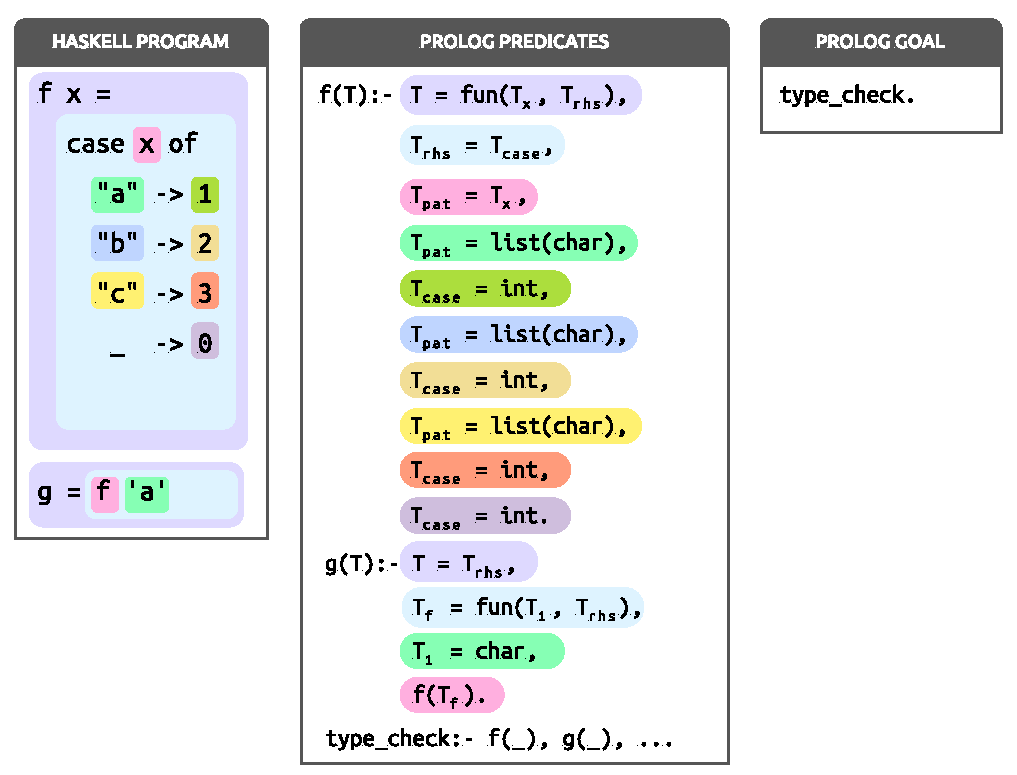
\includegraphics[width=\linewidth]{assets/Translation.pdf}
%     \caption{An example of Goanna generating type constraints.}
%     \label{fig:translation}
% \end{figure}

	\subsection{Post-Analysis}
	Three types of post-analyses are performed by Goanna to improve the quality of error diagnoses: type error grouping, cause ranking, and cause reduction. 
    \subsubsection{Type Error Grouping} \label{sub:grouping}

    Type error grouping is a novel feature provided by Goanna. Conventionally, in a type error slicing approach, a type error is represented by a minimal unsatisfiable subset (MUS). With multiple MUSes available, we have the knowledge to be more precise about an ill-typed program. We propose a novel method of representing type errors that aligns more closely with their colloquial meaning.

	Let $U$ denote the set of all Minimal Unsatisfiable Subsets (MUSes) and $C$ the set of all Minimal Correction Sets (MCSes). We define an undirected graph $G$, where each vertex in $G$ corresponds to a minimal unsatisfiable subset $u_i \in U$, and the edges of $G$ connect pairs of MUSes $u_i$ and $u_j \in U$ if their intersection is non-empty. The set of all connected components $D$ in $G$ represents the set of all type errors. For each $d_i \in D$, let $l_i = \bigcup v_i$, where $v_i$ is the set of vertices in $d_i$. $l_i$ is the set of all constraints local to this type error. Define $C_i = \{ x \mid \forall c \in C, x = c \cap l_i \}$ as the set of all MCSes that are local to this type error.


    This can be intuitively thought of as follows: two type errors can be grouped together if they cannot be fixed independently through modifying a minimal set of locations for each. For instance, Fig.~\ref{fig:grouping-example}.A shows one connected type error, where there are two fixes available: change \texttt{0} on line 1 to a Boolean type, change the type annotation on line 3 to a \texttt{Num} instance, or change the assignment of \texttt{y} to a different expression. Choosing either one will result in both \texttt{x} and \texttt{y} being inferred to have a valid type.
    
    

   \begin{figure}[ht!]
        \centering
        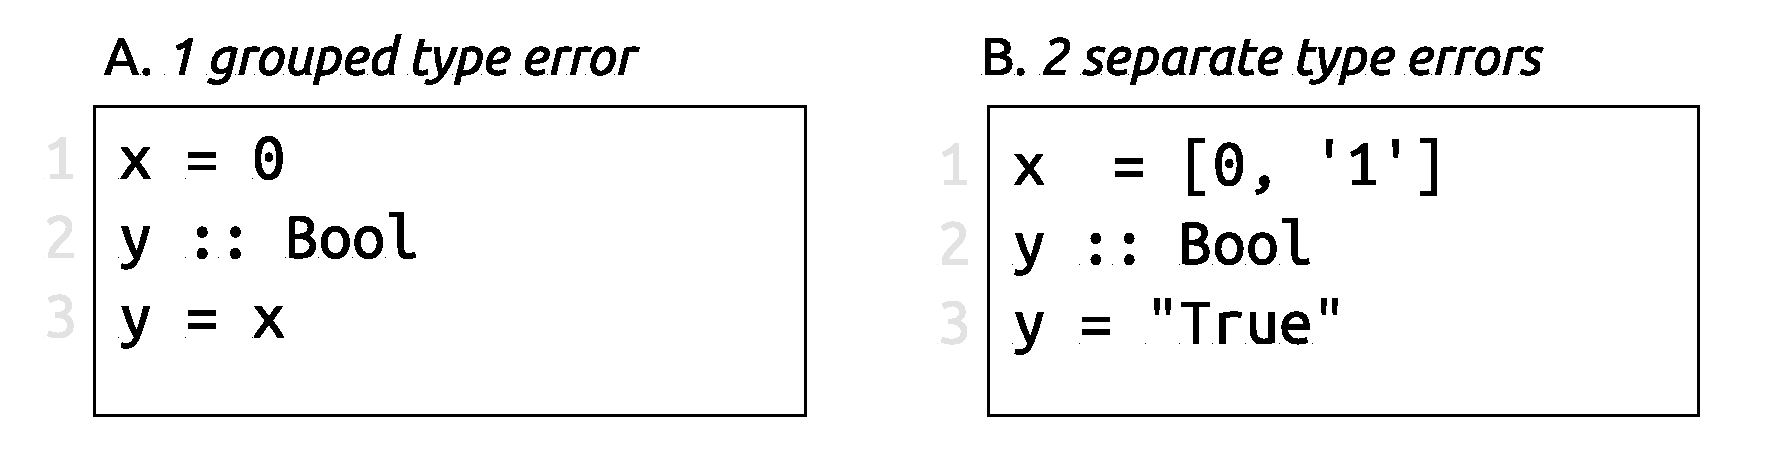
\includegraphics[width=0.8\linewidth]{images/Grouping-Example}
        \caption[Goanna's type error grouping]{\textbf{Goanna's type error grouping.} The ill-typed program on the left contains a single type error, because it can be fixed by a minimal set of syntax changes. For example, fixing it by changing the literal \texttt{0} on line 1 to \texttt{True} or \texttt{False}. This edit contains a single location, so there exists no smaller edit that can fix \texttt{x} or \texttt{y} alone. The program on the right contains two type errors because \texttt{x} or \texttt{y} can be fixed separately. For example change \texttt{0} to \texttt{'0'} on line 1 fix \texttt{x} alone. }
        \label{fig:grouping-example}
    \end{figure}



    However, in Fig.~\ref{fig:grouping-example}.B, although the ill-typed fragment is in a single function, we can fix the argument, either \texttt{0} to \texttt{'0'} or \texttt{'1'} to \texttt{1} to eliminate part of the type error. The same goes for the function's result type \texttt{x}. In this case, there are two separate type errors that should not be grouped.

	
	In practice, type error grouping provides a sense of the ``effective area" of a type error. Programmers are commonly bewildered by the fact that changing one place of the program causes an error in a seemingly unrelated area. When refactoring a known correct program, a programmer can change the definition of one variable, and Goanna will show all the locations that require further changes. This works because all the further changes belong to the same type error group, because a single syntax change -- reverting the initial changes -- will result in the program being well-typed once more.
	
	More specifically, to Goanna, type error grouping provides an effective means to reduce the number of causes. In an ill-typed program with $m$ errors, each having $n$ potential causes, will result in $nm$ total causes. Dividing these causes into separate errors that align correctly with intuition is the most important technique to enhance Goanna's error reporting.

    \subsubsection{Cause Ranking} \label{sub:ranking}
     In Goanna-IDE, when a list of potential causes is on display, Goanna-IDE also shows the top 3 ``likely" causes according to the ranking heuristics. This is very helpful because programmers will have a starting point for the investigation. We provide a set of efficient heuristics for ranking suggestions. 

    \paragraph{Number of Error Locations.}
    Causes comprising fewer locations are prioritized and presented earlier in the list. For instance:
   \begin{figure}[ht!]
        \centering
        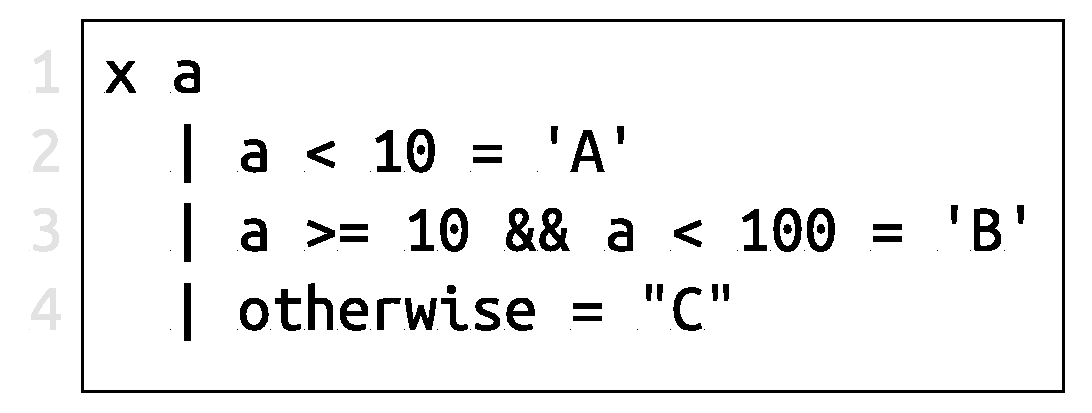
\includegraphics[width=0.5\linewidth]{images/Loc-Count}
        \caption[Goanna prefers causes with fewer error locations]{\textbf{Goanna prefers causes with fewer error locations.} In this ill-typed program, Goanna chooses to give the cause \texttt{"C"} on line 4 a higher likelihood because it contains a single location. The other cause contains 2. }
        \label{fig:loc-count}
    \end{figure}

    In the example in Fig.~\ref{fig:loc-count}, there exist two possible fixes: 1) Changing \texttt{'A'} and \texttt{'B'} to the string type, and 2) changing \texttt{"C"} to the \texttt{Char} type. As the latter fix affects only 1 location (as opposed to 2 in the former), it is assigned a higher ranking and appears earlier in the list.

    \paragraph{Change specificity.}
	Another useful heuristic is to encourage the cause whose fix will result in every surrounding term to be as concrete as possible.
	
	
   \begin{figure}[ht!]
        \centering
        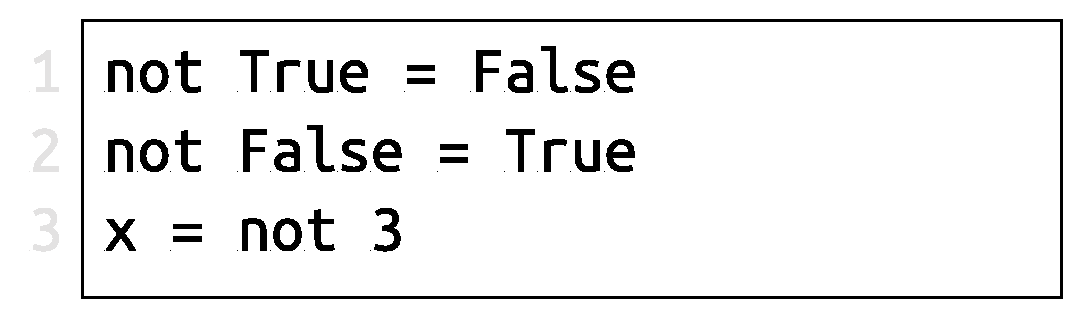
\includegraphics[width=0.5\linewidth]{images/Specificity}
        \caption[Goanna prioritize causes whose resolutions lead to more concrete type assignments]{\textbf{Goanna prioritize causes whose resolutions lead to more concrete type assignments.} In this example, change \texttt{3} will result in \texttt{x} to have type \texttt{Bool}. Alternatively, \texttt{x}'s type will be unknown after changing \texttt{not} on line 3. Goanna prefers the former.} 
        \label{fig:specificity}
    \end{figure}

    In the example in Fig.~\ref{fig:specificity}, Goanna can suggest two potential causes and fixes. First, change the integer literal \texttt{3} to a \texttt{Bool} type. Second, change the function \texttt{not} to a different function that accepts an integer as input. The second fix results in variable \texttt{x} having a less concrete type. Indeed, \texttt{x} can have any type if not limit what function to replace \texttt{not} with. Goanna prioritizes the first cause over the second. 

    \paragraph{Error span.}
    Goanna prioritizes the potential causes whose corresponding locations are clustered within fewer function definitions and lowers the likelihood of those whose corresponding locations are spread across multiple definitions or even multiple files.  

    
    \subsubsection{Cause reduction} \label{sub:optimization}
    
    We employ three techniques to elevate the clarity of the suggestion list: reduction of constraint count, elimination of over-fitting resolutions (solutions that are technically correct but involve making unnecessary modifications), and elimination of redundant fixes.

    \paragraph{Minimize Constraint Count.}
    The number of constraints directly influences the time complexity associated with enumerating the Minimum Correction Subset (MCS). By merging multiple constraints into a singular one, we can reduce the total count of constraints and, in turn, improve the performance of enumeration. Yet, this approach requires careful application, as it could potentially lead to unsolvable situations or propose infeasible fixes, as the combined locations in the source code must either all contribute to the type error or none do. An effective application of this technique is to merge all constraints created by sub-expressions in a type signature.

   \begin{figure}[ht!]
        \centering
        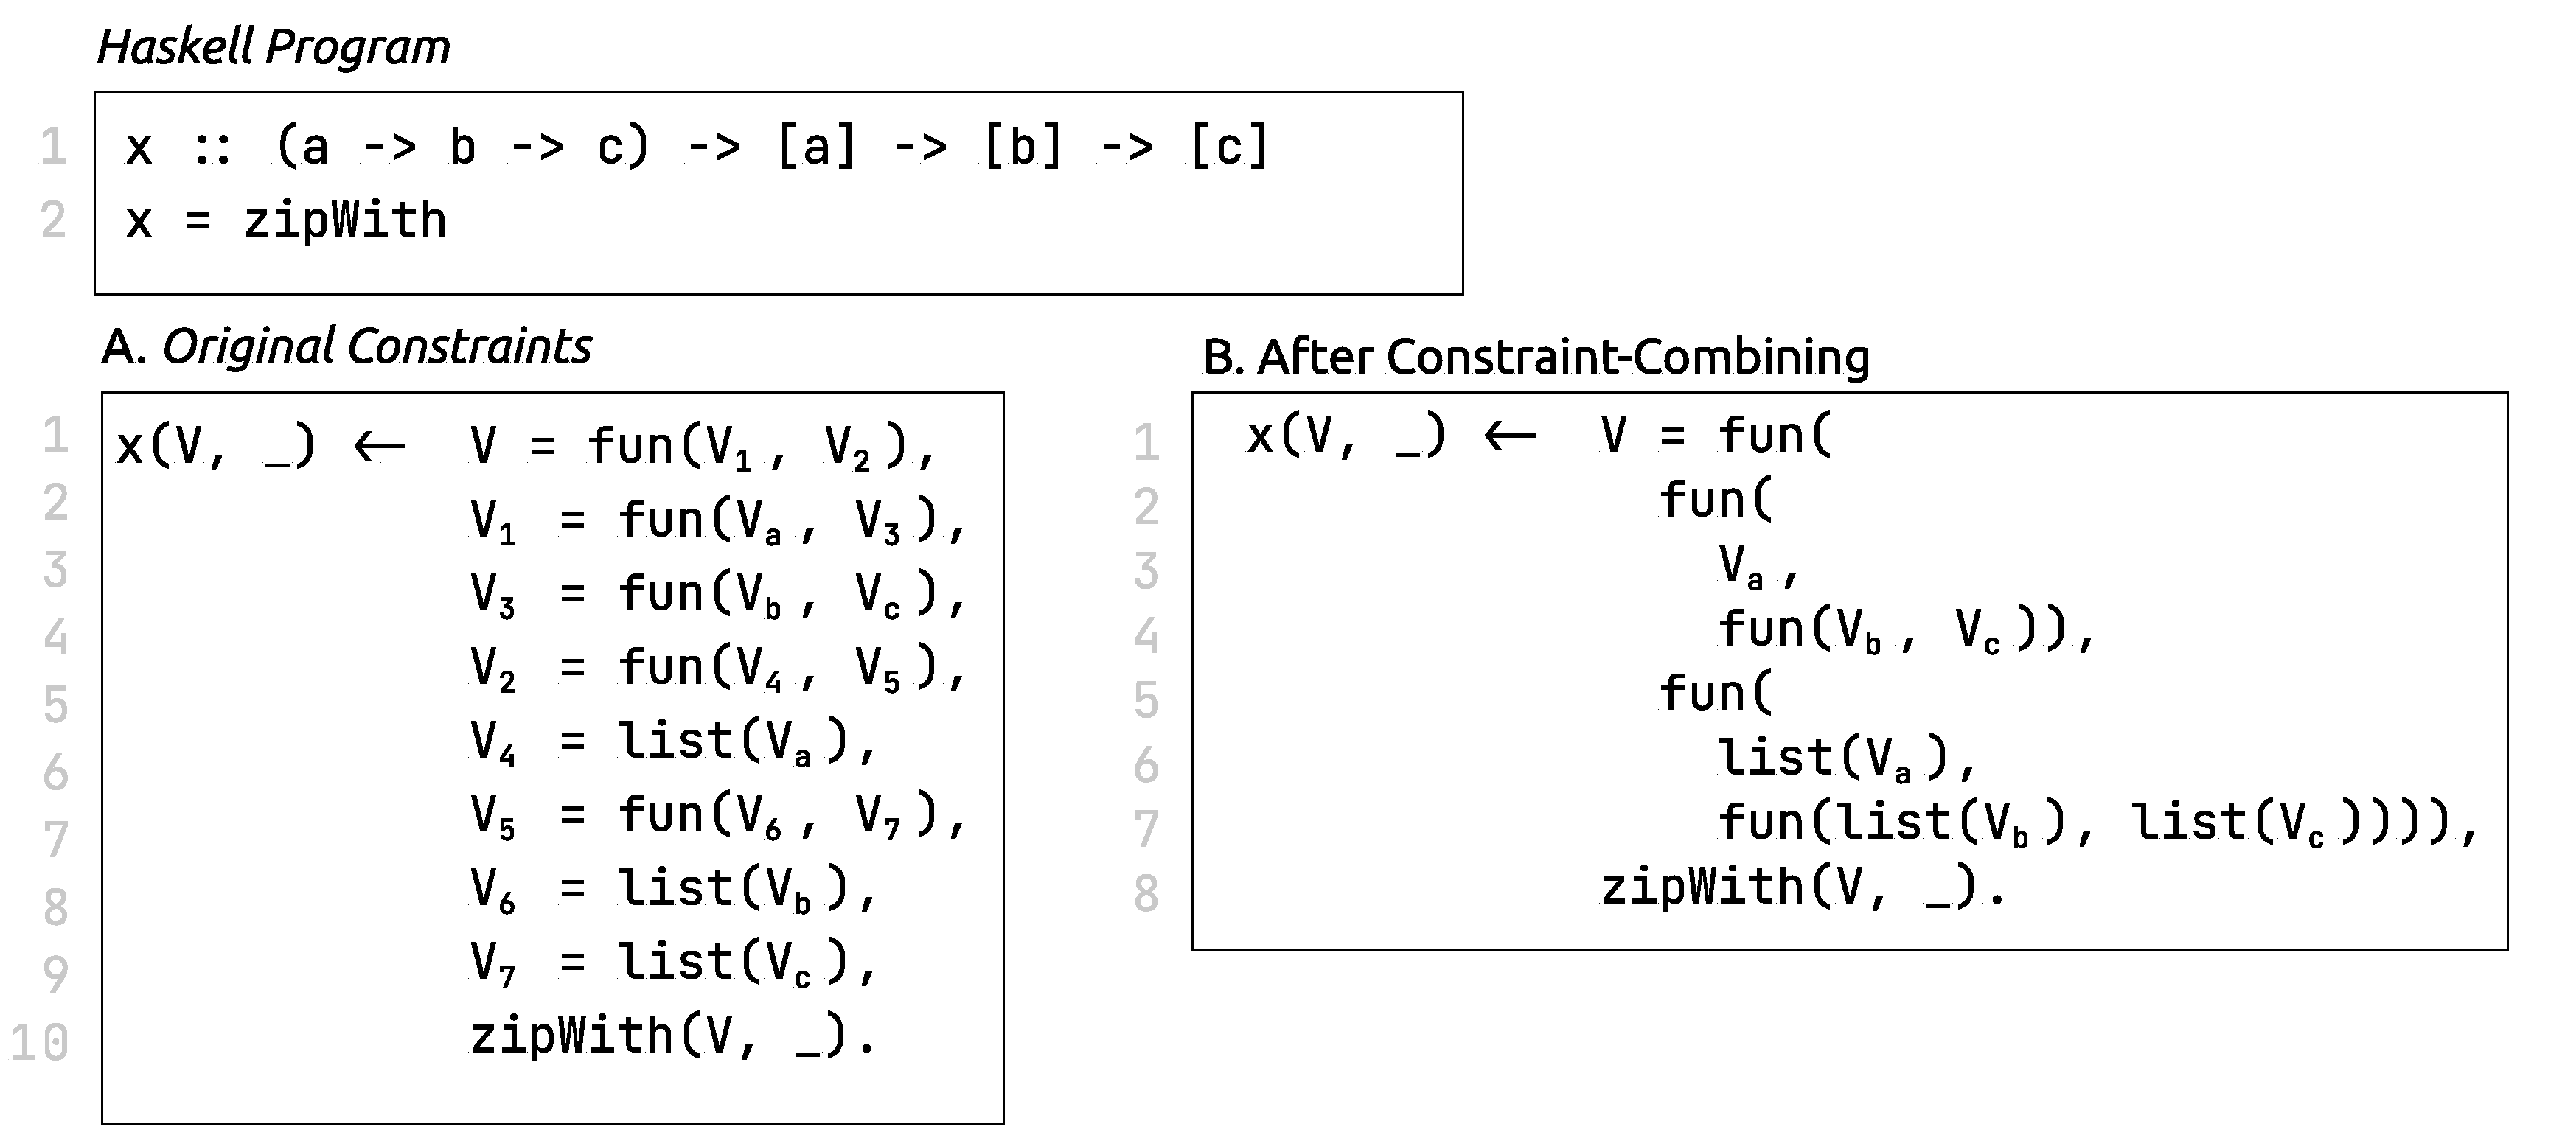
\includegraphics[width=\linewidth]{images/Combine-Constraints}
        \caption[Combine constraints in type signature]{\textbf{Combine constraints in type signature.} For a simple Haskell program (top),  without any optimization, Goanna generates 10 constraints (bottom left), indicated by 10 subgoals in the predicate. By combining the constraints in the type signature, Goanna produces 2 constraints (bottom right).}
        \label{fig:combine-constraints}
    \end{figure}

    Consider the example in Fig.~\ref{fig:combine-constraints}. Without optimization, this code would spawn 10 constraints. However, applying this optimization can achieve an equivalent outcome with merely 2 constraints. Notably, this optimization forfeits the capability to suggest fixes for sub-expressions within a type signature, a decision that warrants some consideration but, in our experience, pays off.

    \paragraph{Elimination of Over-Fitting Resolutions.}
    Over-fitting often refers to a situation where error correction tools provide solutions that are technically correct but involve making unnecessary modifications. In Goanna, every syntax node in the source code generates one or more constraints. This includes structural nodes such as function applications and let expressions. However, very often, suggesting that the user should modify the entire function application expression is not particularly instructive when changing one of the arguments fixes the type error as well. Disabling suggestions for over-fitting solutions improves the clarity of the suggestion list and enhances the speed of MCS enumeration.
   

    \paragraph{Elimination of Redundant Causes.}
    Goanna iterates over the possible causes and removes the ones that fail to deliver new insights. If all locations in a cause suggestion have already been covered in preceding suggestions, subsequent suggestions that merely rearrange these locations in different combinations can be omitted.
    
   \begin{figure}[ht!]
        \centering
        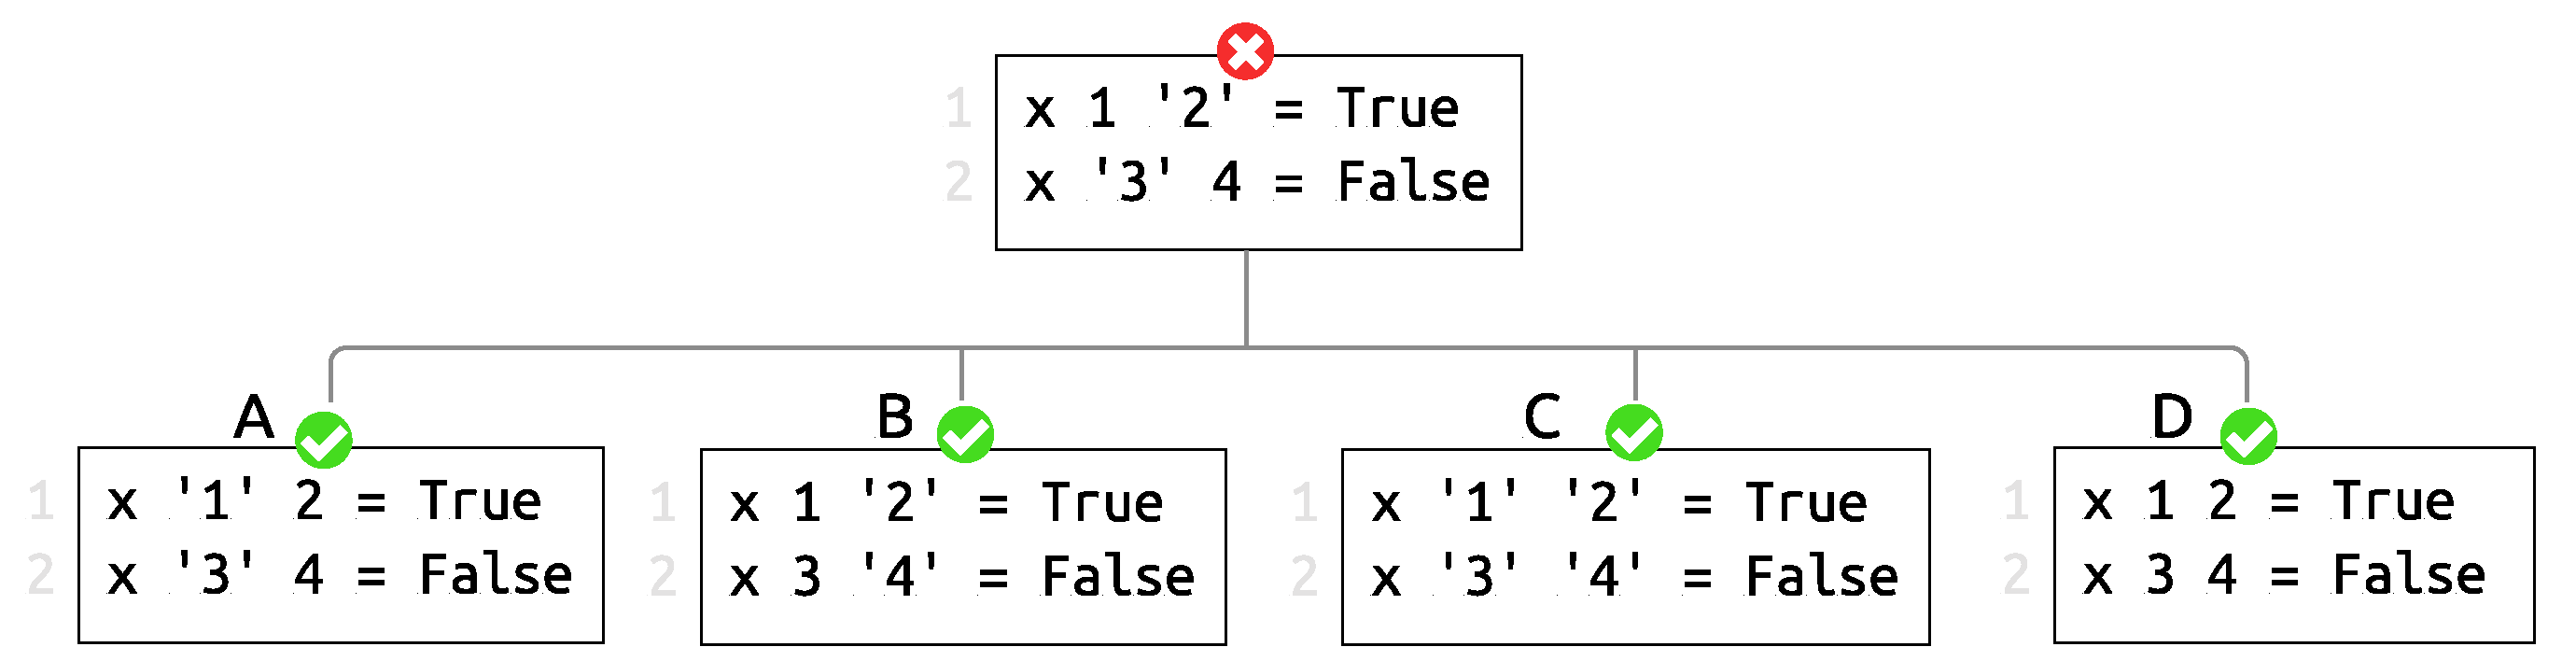
\includegraphics[width=0.9\linewidth]{images/Reduction-Example}
        \caption[The number of potential causes can grow exponentially]{\textbf{The number of potential causes can grow exponentially.} In the ill-typed Haskell program (Top), there are 4 different ways (Bottom) to fix the type error. It is not hard to see this growth is exponential, and showing all the alternatives is not helpful.}
        \label{fig:reduction-example}
    \end{figure}
    
    Consider the example in Fig.~\ref{fig:reduction-example}. Without knowing the true intention of the programmer, Goanna can provide four ways to fix the issue shown at the bottom. However, closer inspection reveals that after the first two suggestions, we no longer unearth new insights. Therefore, they can be removed to enhance the clarity of the suggestion list. 
    Note that this can remove the correct answer (say D), but if the programmer uses part of the (A) to make the fix, the revised type error will include the correct fix. 
    
    Removing superfluous MCS-based suggestions that recycle different permutations of the same set of locations is an instantiation of the Set Cover Problem (SCP). The problem can be rephrased as finding the minimal number of MCSes that cover all the potential locations that could cause the type error. Many approaches solve the SCP \cite{Caprara2000-vw}, including eager algorithms, linear programming, and heuristic-based algorithms. Generally, we found all of these approaches find the minimal cover of type errors efficiently. Goanna uses the OR-tools \cite{Google_Developers_undated-ew} for this task.
       
    \section{Evaluation} \label{sec:evaluation}

     We want to answer the following key research questions about our Goanna prototype:

    \begin{itemize}
        \item RQ1. Does Goanna provide a more accurate type error diagnosis compared to traditional tools?
        \item RQ2. Does Goanna provide a concise list of suggestions?
        \item RQ3. How efficiently does Goanna compute error diagnoses?
    \end{itemize}

    \subsection{Experiment Design} \label{sub:dataset}

    To assess Goanna, we extracted a collection of defective Haskell programs (N=86) from Haskell online discourse since 2018, each containing one or more type errors. The communities we searched include StackOverflow (32), Haskell on Reddit (20), and Haskell Discord Channel (34), as these are the top discussion channels for Haskell users \cite{Fausak2022-zf}. During the search process, we looked for online discussions where the authors encountered type errors in their Haskell programs and asked for help. Further, we selected only the questions that had been answered and accepted by the original author. We extracted the defective Haskell programs and the accepted answers as the oracle solution. The length of these programs ranges from 1 liner to 64 lines of code (mean=20, median=20). These programs span a variety of subjects, including basic syntax (14 files), lists (28 files), tuples (5 files), algebraic data types (22 files), higher-order functions (17 files), monadic operations and do notation (9 files), type classes (6 files), and built-in/library functions (24 files). The distribution of themes generally aligns with the breakdown of the different causes of the type errors from Tirronen's study \cite{Tirronen2015-nr}.
    
    	For each metric in the evaluation, Goanna is compared with Glasgow Haskell Compiler (GHC) \cite{Gamari_undated-zu}, and Helium \cite{Hage2023-kk}. GHC was chosen as the baseline due to its established reputation in the Haskell community, wide capability, and great efficiency in working with Haskell projects. Helium is acknowledged for producing high-quality error messages \cite{Heeren2003-kd}. The experiments were run with GHC 9.4 and standalone Helium compiler version 1.8.
    
    


 	\subsection{RQ1. Accuracy}\label{sub:eval-accuracy}
 	For each program in our dataset, we compared each tool's error diagnosis with the accepted answer. We consider the diagnosis accurate only if its suggested fix matches the accepted answer. We consider the diagnosis partially accurate if the tool's diagnosis is part of a larger set of locations that make up the intended cause or if the diagnosis addresses one of the multiple errors. Because Goanna provides a comprehensive list of possible causes, it is very likely all sensible fixes are included. In this evaluation, we only consider the top-1 suggestions (Goanna 1) and top-3 suggestions (Goanna 3).  From the graph in Fig.~\ref{fig:accuracy}, GHC's accuracy is the least performant among all tools. Goanna 1's, although lower than Helium (72.1\%) in partial accuracy, is higher than Helium (51.2\%) when considering only diagnoses that fully match the accepted answer. \textbf{Goanna 3 has the best accuracy (84.8\%)}, higher than the partial accuracy of other tools.
  
     \begin{figure}[ht!]
        \centering
        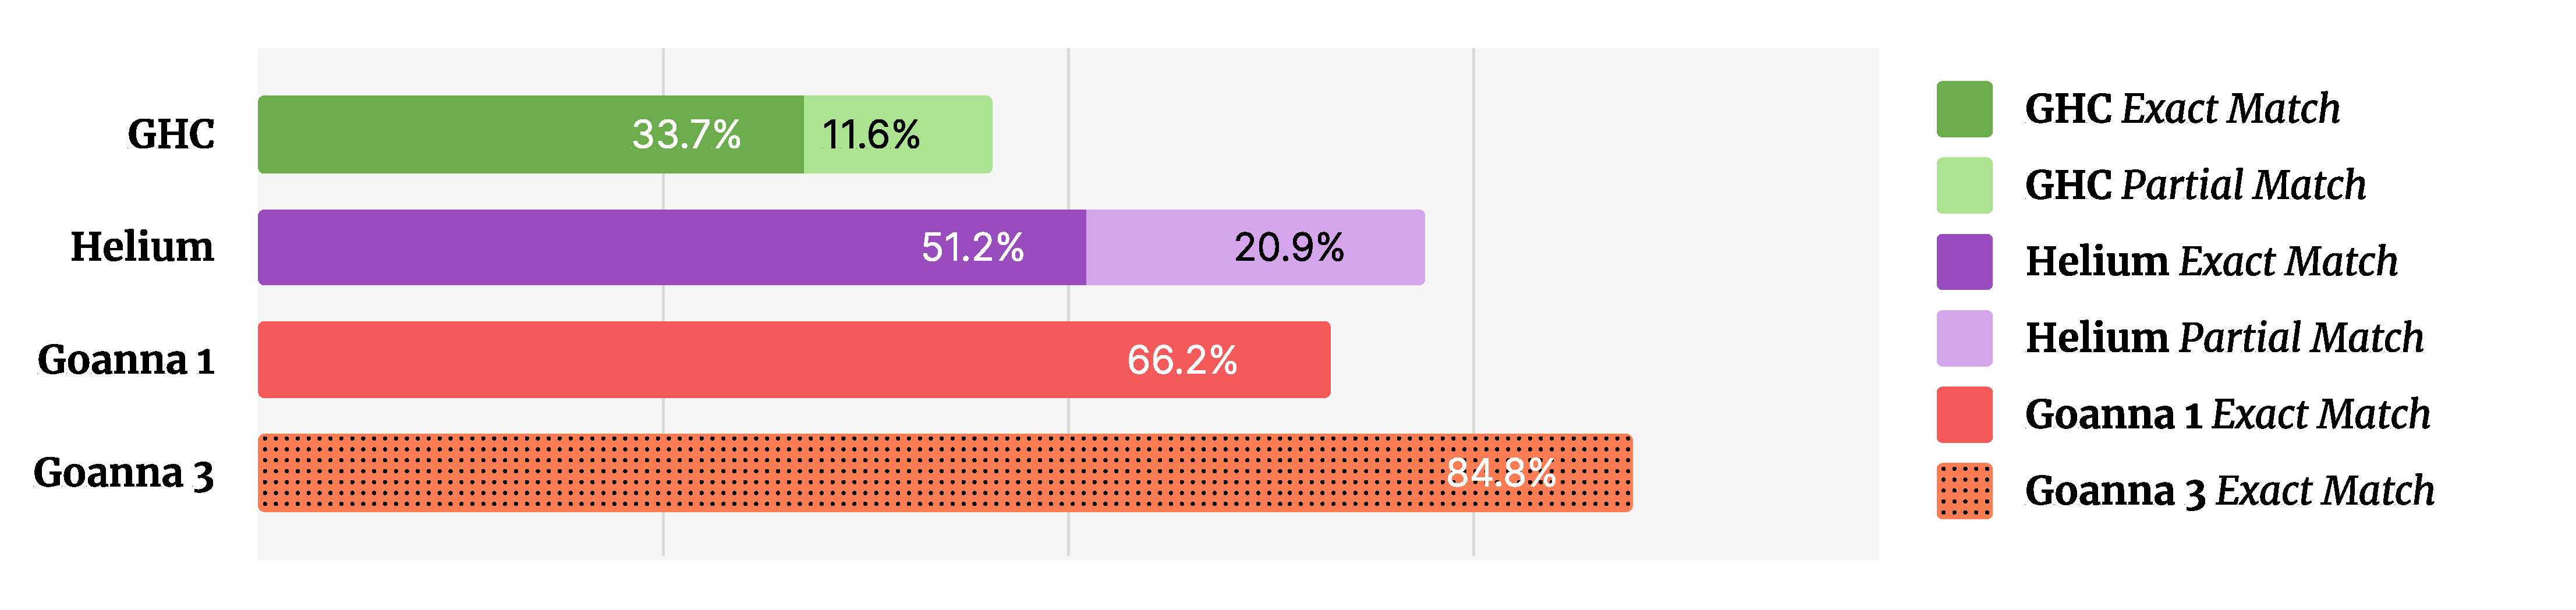
\includegraphics[width=\linewidth]{images/Accuracy}
        \caption{The percentage of diagnoses that match the accepted answers.} 
        \label{fig:accuracy}
    \end{figure}


 	


 	\subsection{RQ2. Conciseness}\label{sub:eval-conciseness}
 Using Goanna requires users to cherry-pick from a list of possible causes. It will severely reduce the usability if the list is too long. To evaluate Goanna's conciseness, we counted the number of suggestions provided by Goanna in all the tasks.  We also indicate where the accepted answer is. Additionally, we included a baseline of Goanna with all the cause reduction features disabled. As shown in Fig.~\ref{fig:conciseness}, \textbf{Goanna manages to effectively condense its suggestion list}, on average providing a short list of suggestions (mean=3.29, median=3.0) for each type error. Additionally, on average, the accurate cause can be found within the top 2 suggestions (mean=1.63, median=1.0) to find the correct cause identification and fix. It also shows in Fig.~\ref{fig:conciseness} that Goanna's cause reduction strategies are effective; on average 51\% of total causes are reduced to gain clarity. One unusual observation is that in 3 tasks, Goanna failed to include the correct solution. The current version of Goanna is ineffective in making the correct suggestions for these type errors. We discuss this in Section~\ref{sec:edge-case}. 
 
    \begin{figure}[ht!]
        \centering
        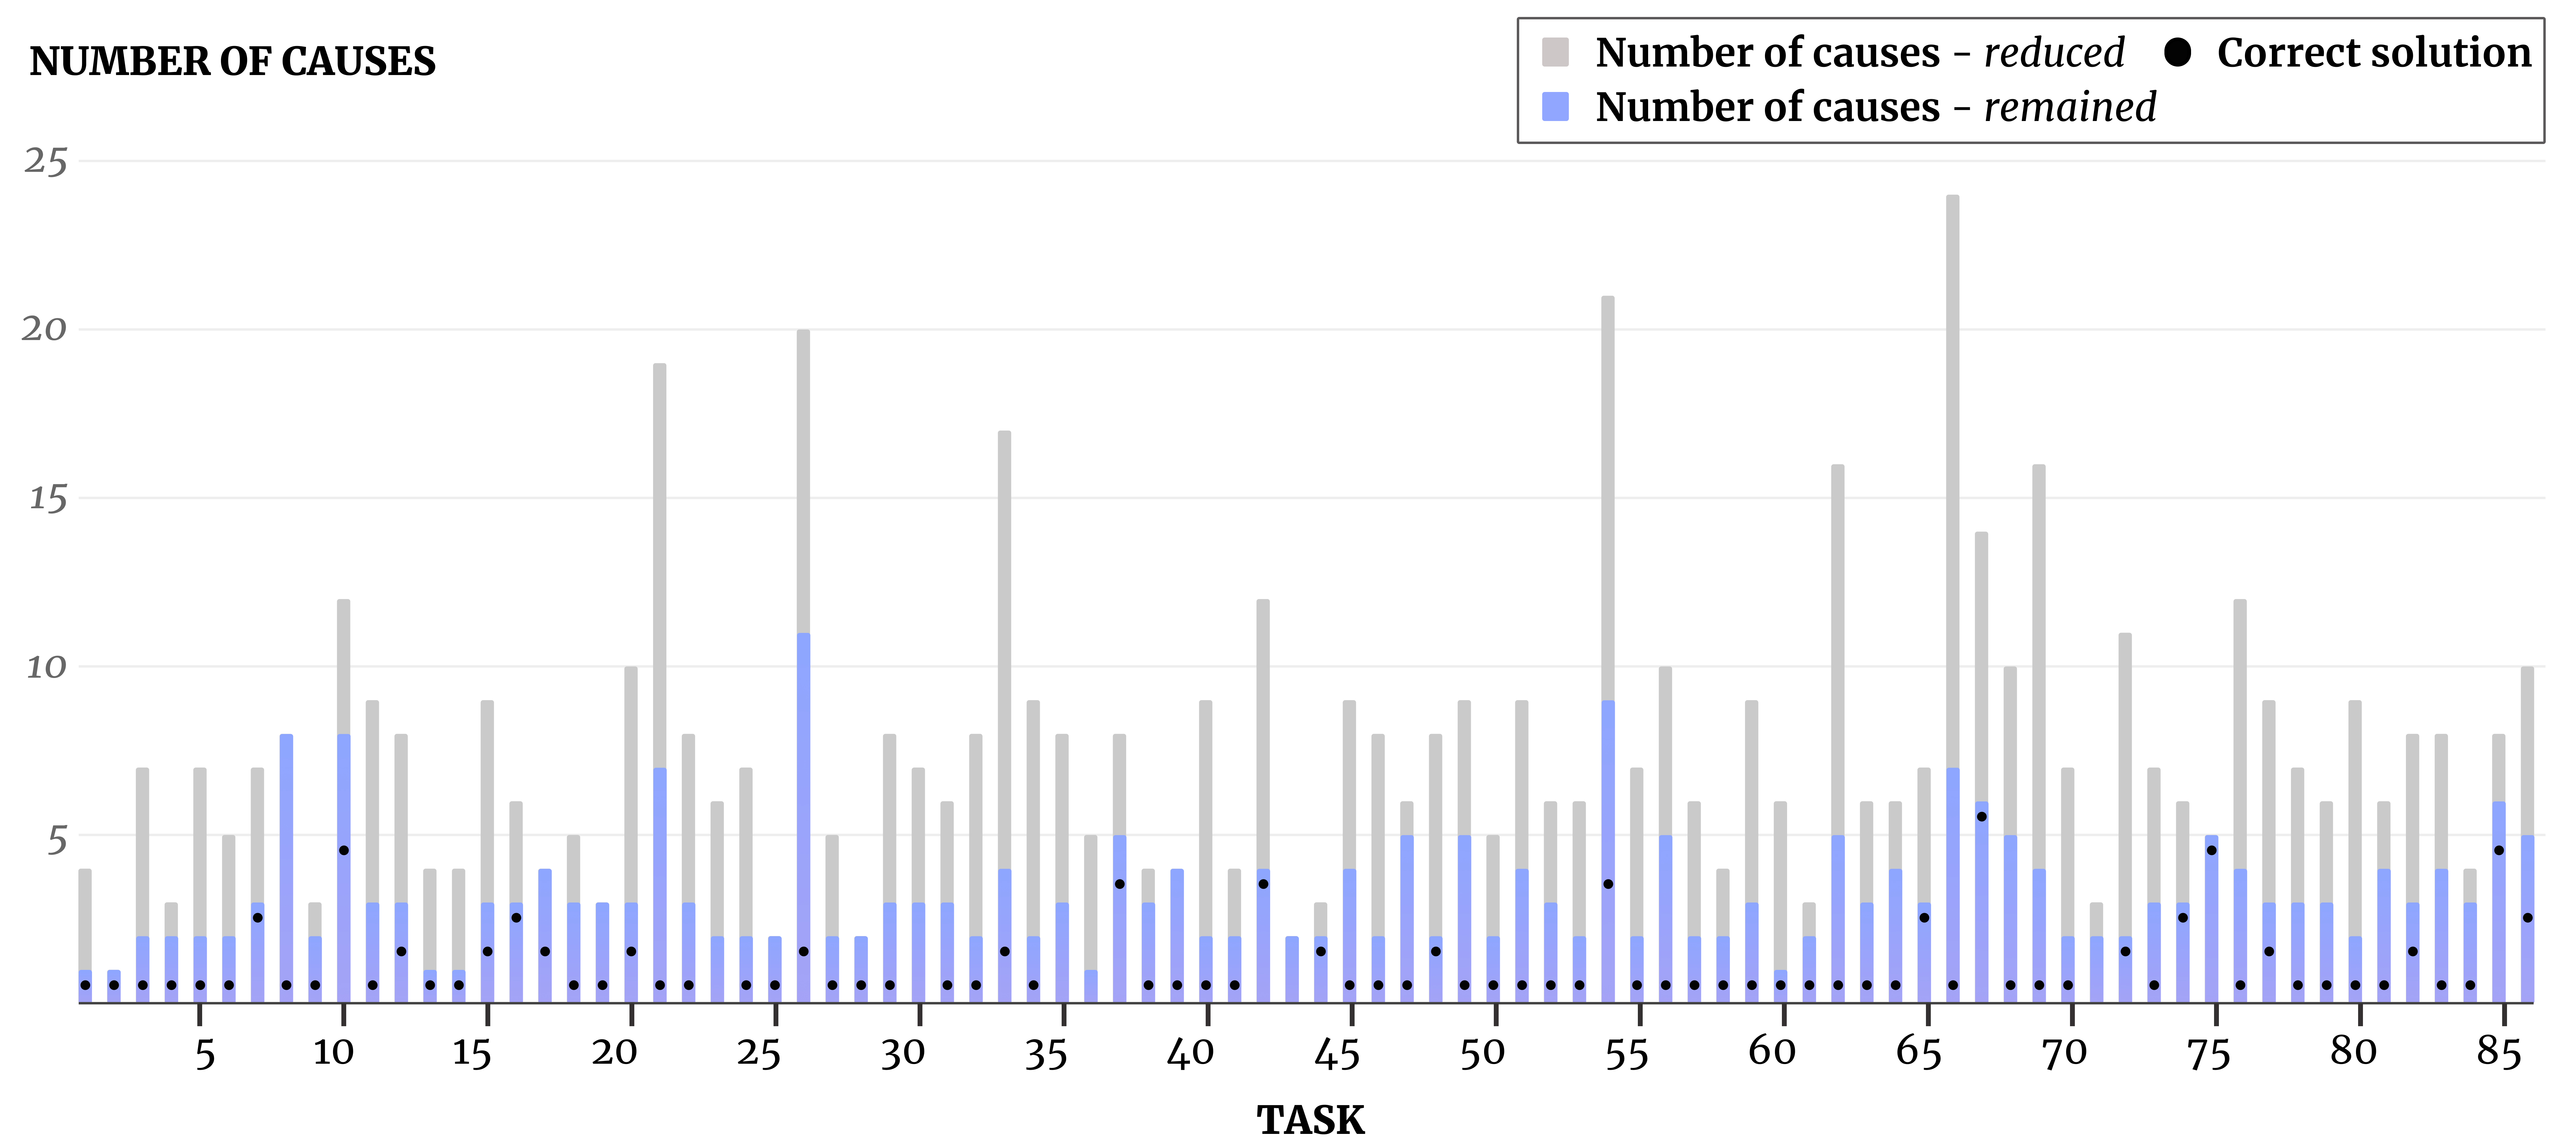
\includegraphics[width=\linewidth]{images/Conciseness}
        \caption{The number of potential causes identified by Goanna.}
        \label{fig:conciseness}
    \end{figure}



    \subsection{RQ3. Performance} \label{sub:eval-performacne}

    Goanna's performance largely depends on the MCS enumeration phase. Enumerating all MCS is computationally expensive. We experimentally compared the time it takes for Goanna to provide a complete error diagnosis for each task with GHC and Helium. From the data shown in Fig.~\ref{fig:performance}, we can see that \textbf{Goanna is slightly slower than Helium}~(Goanna: mean=0.98 seconds, median=0.83 seconds; Helium: mean=0.63 seconds, median=0.63 seconds). Goanna is about 10 times slower than GHC (mean=0.09 seconds, median=0.09 seconds), but greatly outperforms GHC (see Fig.~\ref{fig:accuracy}). One important pattern is that Goanna's response time varies more than other tools (Goanna SD = 0.55, GHC SD = 0.00, Helium SD = 0.10). It can be seen from Fig.~\ref{fig:conciseness} and Fig.~\ref{fig:performance} that the tasks Goanna struggles most with are the ones that have significantly more potential causes. Multiple avenues exist to mitigate this delay, and we discuss them in Section~\ref{sec:future-work}.
    
    \begin{figure}[ht!]
        \centering
        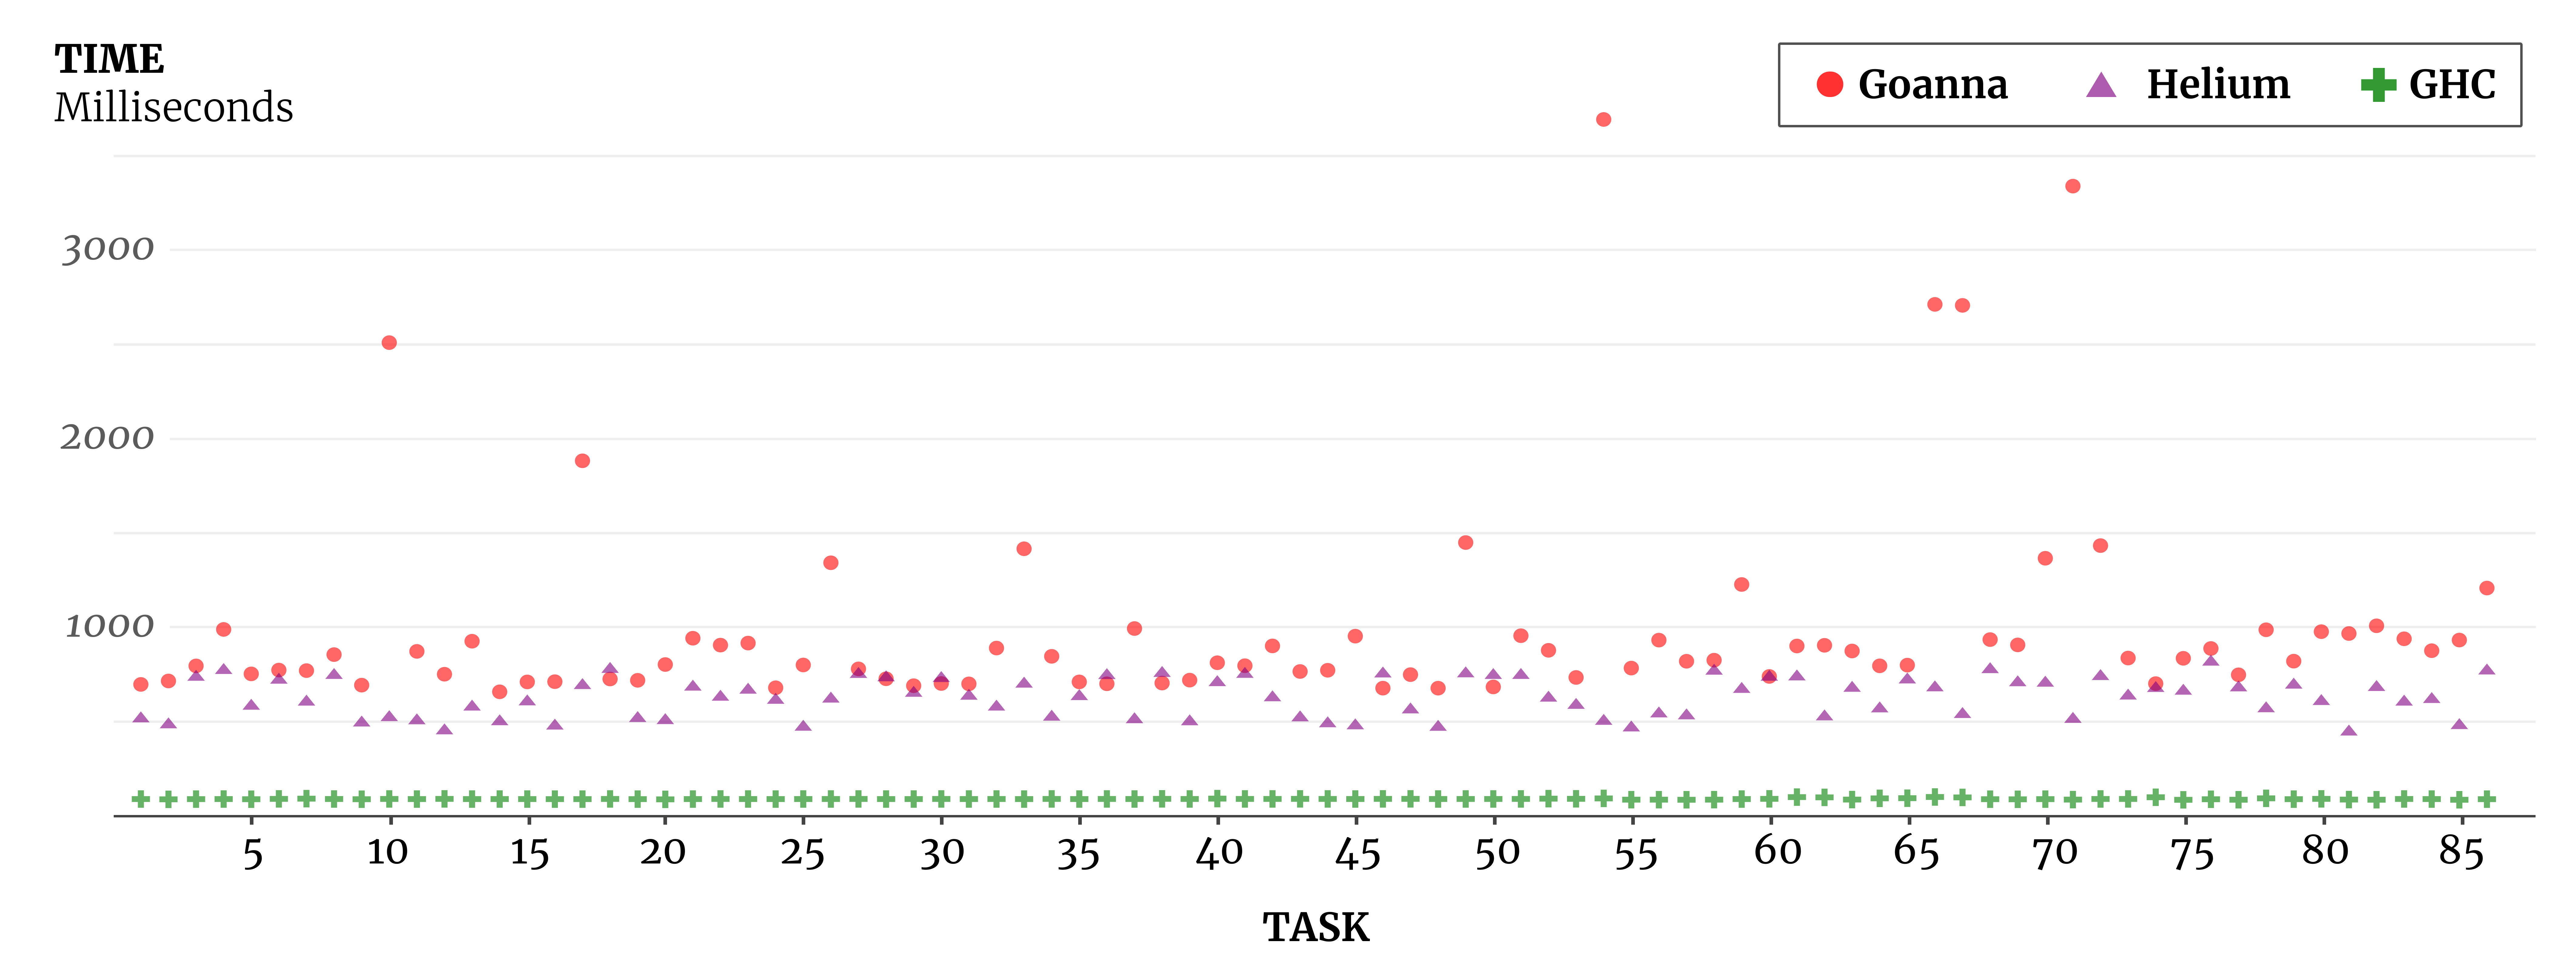
\includegraphics[width=\linewidth]{images/Performance}
        \caption{The time it takes to type check and diagnose each program.}
        \label{fig:performance}
    \end{figure}

	
	
% \todo{can you show a graph of some sort?}

% \todo{Any user evaluation...? Even if a preliminary one/small numnber experts would greatly help...}

% \subsection{Qualitative Results}

    \subsection{Threats to Validity}

    \paragraph{\textbf{Selection of the dataset}}
    Our selection of dataset is limited in its number. This is due to the challenge of finding programs that contain type errors. Unlike runtime errors, which can be mined from code repositories and version control histories, type errors in Haskell can be detected by the compiler tool, and ill-typed programs are usually fixed before the changes are committed to the version control systems. Further, we employed two selection methods. First, the error is indeed a type error. We test this by running the original program in GHC and checking if it indeed triggers a type error. The program is discarded otherwise, for instance, if it contains only parsing errors or runtime errors. Second, we discarded type questions where the main error relies on third-party libraries. 
    
  
        
    \paragraph{\textbf{Measurement of performance}} Performance on Goanna and GHC was measured on a Linux virtual machine with a 3.1 GHz Processor and 2GB RAM. In practice, complex systems like this may perform differently depending on hardware and software configurations. Although we were not able to extract the performance profile of each tool across different platforms and operating systems, we chose hardware with abundant resources and up-to-date software dependencies. During our performance measuring, neither CPU usage nor memory usage was fully stressed. Additionally, GHC was run with the ``-fno-code'' flag enabled to limit its usage to type-check only.


    \section{Discussion} \label{sec:discussion}

    Drawing on the evaluation's findings, we identify Goanna's strengths and weaknesses. We propose directions for future work to provide useful applications and address its current limitations.

    \subsection{Strengths}
    Goanna demonstrates notable improvement over existing Haskell type error detection and repair tools. Compared with traditional type-checking tools such as GHC, Goanna delivers improved error detection accuracy and flexibility to inspect different potential causes. The data suggest that users typically need to consider only 2-3 suggestions to achieve a satisfactory result. It improves error localization organization, avoiding the presentation of all error locations at once.


    \paragraph{\textbf{Accurate suggestions}} Goanna is able to identify causes for Haskell type errors more accurately than GHC and Helium. We attribute this to a few factors. First, Goanna is the only tool capable of suggesting the type error in more than one node. In a study on how students fix Haskell type errors~\cite{Wu2017-eb}, of over 2700 ill-typed Haskell programs, only 35\% of the type errors were caused by a single location. However, most of the type debugging tools only focus on single-location causes due to their technical limitation or to avoid high computational cost. Second, Goanna is the only tool that provides alternative causes of a type error. We were able to see that although Goanna-1 is not as accurate as Helium when accepting partial fixes, Goanna-3 surpasses Helium in accuracy. This translates into accurate type error identification at the cost of presenting the top 3 answers from Goanna instead of one.
    

    \paragraph{\textbf{Goanna provides contextual information}}
    Goanna provides type information for relevant terms to support each of its claimed causes. In traditional tools, the type-level information is often incomplete or totally discarded. In runtime error debugging, one of the most common features is inspecting the values of different expressions of the program. It would be ineffective if the runtime debugger only showed the location of the error. Goanna simulates this feature in the type debugging setting. Instead of run-time values, Goanna allows programmers to inspect the type assignments and observe how they change with different assumptions of the potential cause of a type error. 

    \subsection{Weaknesses}

    The current implementation of Goanna also has a few drawbacks. We provide two: its moderate performance and its tendency to misunderstand the type of error in some edge cases. 
    \paragraph{\textbf{Responsiveness}}
    The trade-off of extensive analysis undertaken in Goanna results in a substantial delay (mean=0.98s).
    The current performance of Goanna is not yet suited for real-time feedback in programming tasks. Based on Nielsen's suggestion for wait time tolerance \cite{Ferdowsi2023-au}, Goanna should provide responsive answers ($\leq$ 1 second) for real-time programming analysis, where users' flow of thoughts stays uninterrupted. Even in larger and more complex tasks, Goanna's response time ($\leq$ 10 seconds) is still suitable as an on-demand tool when a complex type error occurs. As shown in Wu's study \cite{Wu2017-eb}, in the simplest situation where students fix the type error in a single step, it will usually take about 60 seconds to complete the task. This error resolution time grows in proportion to the number of steps the students take to fix the error. If Goanna is able to shorten the steps to final resolution, then the querying time will easily be offset by the time it saves.

    \paragraph{\textbf{Edge cases}} \label{sec:edge-case}
    Although Goanna's error reporting is, in general, exhaustive, there are situations where Goanna still fails to provide insightful diagnosis. One general theme is that Goanna is very effective when the error requires modifying a syntax node but can be less insightful when the intended fix is to insert, delete, or rearrange syntax nodes. In the example in Fig.~\ref{fig:weakness}, Goanna suggests changing the \texttt{map} function to a function of type \texttt{[Int] -> [Bool]}. But in practice, a human user would very easily identify that an expression defining the function to be mapped is missing between the map and the list being operated on.
    
        \begin{figure}[ht!]
        \centering
        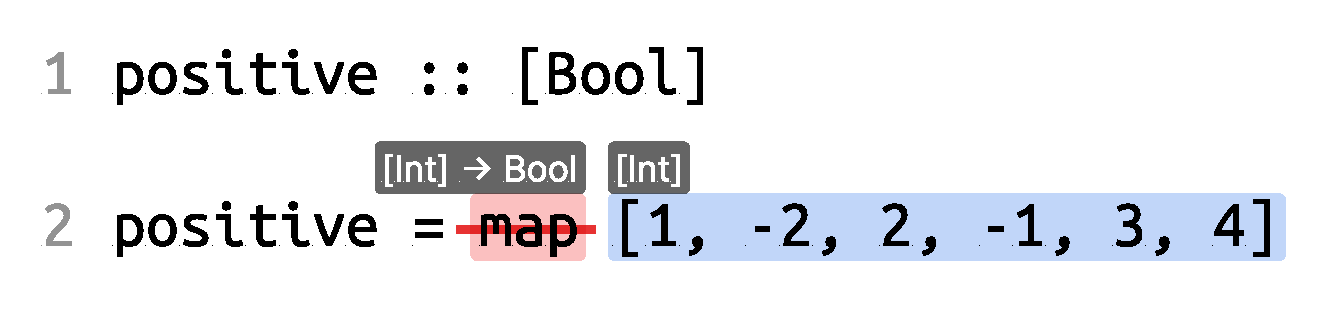
\includegraphics[width=0.6\linewidth]{images/Weakness}
        \caption[Edge cases in Goanna]{\textbf{} In this type error, Goanna suggests changing \texttt{map} to a function of type \texttt{[Int] -> Bool}. Although this is technically correct, in practice, a human expert user would easily identify that a function expression is missing between the function \texttt{map} and the list literal.}
        \label{fig:weakness}
    \end{figure}

%    \paragraph{\textbf{Goanna's suggestions are local}}
%    One potential argument against Goanna's method is its tendency to generate local changes for fixes. Some consider that errors sometimes demand architectural changes rather than localised adjustments. To address this concern, Goanna implements two strategies. Firstly, Goanna presents all relevant error locations in style similar to type error slicing tools and reports all definitions and usages related to a type error. These hints can serve as a mental map to guide the formulation of changes on a large scale and understand their implications at the source code level. Secondly, Goanna consistently provides potential changes in type annotations. A top-level type annotation is a common approach for programmers to map out high-level structures at various stages of Haskell projects. Understanding the required changes at this level enables programmers to adopt a more principled development approach.
%
%	
%	\subsection{Implication}
%	Goanna shows a novel approach to model type errors, and enhances our ability to interrogate them.  Goanna also shows various type error optimization and enhancement opportunities enabled by constraint programming techniques. It suggests more useful programming languages and tools can be developed equipped with MCS-based analysis.
	



% \subsection{Different Category of Type Errors}
% \subsubsection{Where are all the materials}
% \subsubsection{Type errors that involve a long chain of reasoning}
% This kind of type error tend to cause Goanna to report a large number of suggestions. This is easy to understand intuitively because in a long chain of reasoning, breaking any one of them will result in a valid program. So the number of solution should be in propotion to the length of the chain.

\subsection{Future Work}\label{sec:future-work}
  	It is important to evaluate Goanna with human participants and gain qualitative insight into its effectiveness. In one of our workshop preliminary studies, participants show positive reactions after using Goanna. A rigorous human study based on realistic debugging use cases is planned in the near future.   
  	
  	
    Several areas of potential enhancement could improve Goanna's functionality and efficiency. One exciting path of improvement is to generate suggestions for syntax changes on top of type changes. As pointed out by Chen and Erwig \cite{Chen2014-dz}, syntax changes are much more challenging than type changes. But with the recent improvements of generative models and research advancement in ML-based type error \cite{Seidel2017-uf}, accurate syntax changes may be on the path to becoming feasible.

    Several approaches to achieve higher performance of Goanna show promise. The parallel capability of state of the art MUS enumeration \cite{Zhao2016-bu} algorithms are not explored in this study. With proper implementation, it will be possible to lower the hardware barrier of entry for wide adoption of MCS-based type error suggestion tools. Further, with domain-agnostic MUS enumeration tools \cite{Bendik2020-pz}, it should be possible to consistently achieve high performance while using a more performant constraint system and proper parameterization. Lastly, in a real-world implementation, it is possible to employ partial MUS enumeration \cite{Previti2013-mr,Liffiton2016-xi} to restrict the enumeration process in a sensible time-bound.

    Additional future work could include examining Goanna's integration with other tools within the Haskell development ecosystem. For instance, including Goanna in widely used text editors or development environments could offer a more integrated and fluid experience for developers and an important avenue for Goanna to reach a wider audience. 

    Finally, it may be important to consider extending Goanna's capabilities to support other functional programming languages beyond Haskell. Several other languages, including Scala and OCaml, also support static typing and type inference, and Goanna could be a valuable addition in these contexts. In the future, we also hope to extend these techniques to popular multi-paradigm languages such as TypeScript and Rust.


    \section{Related Work} 
    \label{sec:related-work}
    In this section, we survey the corpus of work that Goanna built upon and was inspired by. We first review the work that is built on a theoretical foundation similar to that of Goanna. We then examine studies that share similar aims and offer a comparable debugging experience to Goanna. Finally, we delve into research on program slicing and discuss how Goanna extends the concept of slicing and distinguishing itself from its predecessors.



    \subsection{MCS enumeration}
	
    MCS enumeration has been extensively studied in the field of error localization across various domains. In the specific context of Haskell type error diagnosis and resolution, several related approaches have been explored. It is important to examine the strengths and weaknesses of Goanna in the context of these areas.

    One notable work~\cite{Lamraoui2016-wr} introduced a tool that utilizes the capability of MCS to localize multiple faults and identify software defects using unit tests. Their approach demonstrated the effectiveness of MCS in pinpointing errors within a program. Similarly, Bekkouche conducted a relevant study~\cite{Bekkouche2015-is}  on MCS utilization for locating program errors in while-loop programs. Their findings showed improved efficiency compared to SAT-based approaches. Although showing strength in programming language static analysis, MCS-based fault localization has not been previously applied at the type system level. Goanna distinguishes itself as the first tool to explore this approach within the realm of type error diagnosis and resolution.

    \subsection{Suggesting changes to type errors}
   Seminal~\cite{Lerner2007-yq} uses syntax mutation and binary search to find appropriate syntax changes to program errors. The advantage of Seminal is that it's capable of suggesting direct syntax changes to common mistakes (e.g., mistakingly swapping the order of function arguments). However, it is impossible for Seminal to provide the complete set of all potential fixes. Nor does it guarantee a suggested solution is minimal syntax change.
   
   Counter-factual typing (CFT) \cite{Chen2014-dz,Chen2020-ad} uses a variation-based type system; it is capable of suggesting the correct type for all possible. CFT shares many capabilities with Goanna, CFT is able to suggest multiple-location changes, CFT uses similar ranking heuristics. Goanna is able to produce an in-depth analysis of the ill-type program, such as type error isolation. CFT and Goanna both aim to produce a complete set of potential fixes, Goanna employs a set of effective algorithms to reduce the exponential number of potential fixes without reducing the quality of suggestions. 
   
   SHErrLoc \cite{Zhang2015-xy} uses constraints as the underlying to perform type inference and type error diagnoses. SHErrLoc is able to suggest multiple possible fixes of the type error and rank them based on heuristics. Unlike Goanna's approach of using a general-purpose constraint language, SHErrLoc relies on GHC's internal constraints and then translates them into SCL (a custom-made constraint language). On the technical side, this approach relies heavily on modification of the compiler and does not remain reliable with later GHCs. Most importantly, there is no way to interact directly with the solver. This renders the kind of constraint manipulation in Goanna and SHErrLoc impossible. Goanna is able to perform type reconstruction for ill-typed programs, that is, finding the most concrete types for all expressions for each potential solution using the Maximal Satisfiable Subsets. SHErrLoc focuses on finding the locations only.


\subsection{Type Error Slicing}

Type error slicing \cite{Haack2004-fr} is a technique to identify all necessary locations of a type error that is necessary for programmers to diagnose the root cause. It has been studied in many studies ever since \cite{Tip2001-qn, Heeren2003-kd}. These studies all use Minimal Unsatisfiable Subset (MUS) to ensure the \textit{completeness} and \textit{minimality}. The drawback of type error slicing is that it often produces too many locations.  Chameleon \cite{Stuckey2003-pz,Fu2021-xd} improved type error slicing by allowing programmers to interactively show the partial MUS by choosing their own assumptions. Compared to these tools that base their analysis on a single MUS, Goanna effectively utilizes all possible MUSes. One benefit of enumerating all MUSes is Goanna covers all locations of multi-witness type errors, while Chameleon reports partial locations. This benefit is, however, at the cost of the computational complexity in MUS enumeration. 


% All programming slicing-based tools use MUS as the underlying data structure to narrow down the potential error locations. MUS is very effective in providing an explanation of why there must be an error. But it also suffers from a few drawbacks. First, the size of MUS can grow very large in certain types of projects, in result, reduced usability. Second, MUS omits crucial information that may play an important role in error comprehension. In this chapter, we investigate these drawbacks in detail and describe how we address them using MCS as the underlying data structure for representing type error. We then show how we designed Goanna, an MCS-based type error debugging environment, and how Goanna can better support type error debugging in examples. Lastly, we show how we designed an empirical study to examine the accuracy, conciseness and performance of Goanna.

\subsection{Multi-witness and Multi-party Type Errors}

Although not supporting granular tracing of multi-step type errors as \chameleon{}, Goanna is especially well-equipped for investigating multi-witness and multi-party type errors. This advantage comes from Goanna's ability to enumerate all MUSes. As we discuessed in Chapters~\ref{chap:haskell-type-checking}, multi-witness and multi-party type errors all involve multiple MUSes. For multi-witness type error, Goanna correctly identify all the relevant witnesses. In comparison, tools based on a single MUS, such as \chameleon{}, pick one witnesses from each endpoint, because of the minimality of MUS. In addition, Goanna is also able to divide complex type errors into multiple simpler ones using the type error grouping feature, providing further clarity into the debugging workflows.



%   
%   This type-based approach aims to provide more accurate and meaningful suggestions for resolving type errors. Goanna falls into the latter category, offering type-based suggestions. However, it is important to note that while Chen's approach relies on search-based techniques, Goanna utilizes the MCS as the underlying suggestion representation. This gives Goanna the advantage of providing resolutions that change multiple syntax nodes in a single fix suggestion. Additionally, using MUS enumeration allows Goanna to perform high-level type error diagnoses, such as effectively identifying the number of type errors present and logically grouping them in intuitive partitions.

%    Constraint-based typing rule translation has been exercised in multiple studies. For instance, \cite{Stuckey2003-pz,Fu2021-xd} demonstrated how to translate Haskell typing relations into constraint-handling rules for improved error reporting. Their work aimed to enhance the understanding and identification of type errors by leveraging constraint-based techniques. Similarly, Demoen et al. \cite{Demoen1999-oj} presented an approach for translating Mercury typing constraints into Prolog formulae similar to Goanna's constraint translation system. These studies have shown the potential of constraint-based type systems in providing explainable and diagnostic capabilities. However, many of these works focus on type system modeling and error reporting based on a single MUS, mainly because they were conducted before efficient MUS/MCS enumeration became practical. In contrast, Goanna effectively utilizes all possible MUSes, providing a complete picture of the error and offering enhanced organizational capabilities for better error diagnosis and resolution.
%
%    By analyzing the existing literature on MCS enumeration, type error fix suggestions, and constraint-based typing rule translation, we can gain valuable insights into the distinctiveness of Goanna's approach. Goanna not only explores MCS enumeration in the context of type error diagnosis and resolution but also provides type-based suggestions and leverages the power of constraint-based techniques to offer comprehensive and intuitive error explanations and resolutions. These contributions position Goanna as an innovative tool with the potential to enhance the development process and improve the productivity of Haskell programmers.


\section{Summary} \label{sec:conclusion}
In this chapter, we introduced Goanna, a tool for identifying and resolving type errors in Haskell code. We described the features of Goanna, including its fix suggestions, type error grouping, and identifying multiple type errors. We also discussed our approaches to reduce and reprioritize fix suggestions while maintaining comprehensiveness. Additionally, we walked through the uses of Goanna-IDE, a type error debugging interface for Haskell.

We evaluated the effectiveness of Goanna from a set of 86 diverse Haskell programs and demonstrated its ability to identify and resolve type errors accurately compared to other tools. We also showed that Goanna effectively condenses the list of causes. When a large number of causes is inevitable, Goanna's suggestion ranking heuristics ensures that more useful fixes are prioritized. Goanna currently works with Haskell, but in the future, we plan to extend its MCS-based error diagnosis to work with other strongly typed languages, such as Rust and TypeScript.
